% \hypertarget{optical-lattice}{%
% \section{Optical lattice}\label{optical-lattice}}
% \chapter{Towards an optical lattice for quantum simulation}
% \section{Quantum $\cap$ Complexity}\label{sec:lat-introduction}
% \section{Optical lattices}\label{lat-history}
% % \subsection{Helium's promise}\label{lat-helium}
% \section{Lattice construction at ANU}\label{ssec:lat-motivation}
% \section*{Future work}\label{lat-futurework}



\chapter{Towards an optical lattice trap for helium}
\markboth{\thechapter.
	TOWARDS A HELIUM LATTICE}{}
\label{chap:lattice}


% % \item\todo{Cite https://physics.aps.org/featured-article-pdf/10.1103/PhysRevX.5.011003 ...
	% LG inequality as measure of quantumness/entanglement witness in large systems, new thermodynamics of many-body quantum information...
	% 'macroscopicity similar to cold atom experiments' - contains sideband cooling ref}



	\begin{adjustwidth}{1.5cm}{0cm}
	\begin{flushright}
	{\fontsize{11}{13}\emph{
	``It might be noted here, for the benefit of those interested in exact solutions, \\
	that there is an alternative formulation of the many-body problem:\\
	How many bodies are required before we have a problem? \\
	G.	E.	Brown points out that this can be answered by a look at history.	\\
	In eighteenth-century Newtonian mechanics, \\
	the three-body problem was insoluble.\\
	With the birth of general relativity and quantum electrodynamics in 1930,\\ 
	the two- and one-body problems became insoluble.
	And within modern\\
	quantum field theory, the problem of zero bodies (vacuum) is insoluble.\\
	So, if we are out after exact solutions, no bodies at all is already too many!"}\\
	- Richard Mattuck\footnote{R.
	Mattuck, \emph{A Guide to Feynman Diagrams in the Many-Body Problem}, Dover Books on Physics (1992)}}
	\end{flushright}

	\end{adjustwidth}

\section{The many-body problem}


	In his 1972 essay \emph{More Is Different} \cite{Anderson72}, Nobel laureate Philip W.
	Anderson argued\footnote{Five years later, he was awarded the Nobel Prize in physics for his work on the electronics of magnetic and disordered systems} that the constructionist hypothesis, that one can reconstruct the universe starting from known physical laws,  `breaks down when confronted with the twin difficulties of scale and complexity.' 
	In this he argues that composing a system out of many well-understood pieces with well-understood interactions will eventually give rise to  phenomena in need of `new laws, concepts, and generalizations'.
	Familiar examples in physics include quasiparticles and hydrodynamics, and even atoms, which compress enormous amounts of microscopic information into an effective description based on observed emergent regularities.
	Anderson acknowledges the utility of reductionism by noting that emergent features are always understandable in terms of their microscopic composition.

	A major challenge in science, then, is traversing this bridge between `macro' and `micro'.
	Simulations (on paper or \emph{in silico}) provide the `upward-pointing' inquiry which aim to explain emergent features in terms of elementary concepts.
	The rapid rise of computing power in the latter half of the twentieth century provided a boon to scientists by permitting direct interrogation of previously intractable theoretical models.
	Simulating systems can now be done en masse, in parallel, and with much less human effort than iterations of manufacturing, transporting, and characterizing physical samples.
	The design-build-test-learn cycle thus contracts, and humankind grows more proficient at the design of compounds or materials with desirable properties such as their light-harvesting efficiency or efficacy at neutralizing certain pathogens.
	In the quantum-mechanical context this project is particularly challenging because analytical models at the microscale may be conceivable but are often analytically intractable.
	
	Further, the amount of information stored in a quantum state, and the computational effort required to forecast its evolution, quickly become so large as to exhaust even the largest supercomputers.
	It was in 1982 that Richard P.
	Feynman laid out a proposition for the now-burgeoning field of \emph{quantum simulation}:
	If you care about the physics, you care about the Hamiltonian.
	The hope, then, is that one can engineer \emph{quantum} systems that behave like a certain other, potentially hypothetical, system of interest and obtain useful data from it more efficiently than via conventional computing, when the cost is measured in some combination of time, energy, or some other convenient currency.
	One flourishing branch of this field of inquiry is the use of \emph{optical lattices} to synthesize artificial crystals, scaled up some 10,000 times and many orders of magnitude colder than conventional solids.
	The ultracold atoms in such systems then play the role of electrons bound in the ion lattice of solid systems.
	Ultracold metastable helium offers a dramatic extension of the questions one can ask of optical lattice simulators.

	In this chapter I discuss efforts towards constructing an optical lattice trap for helium.
	I will describe the motivation for the project and some calculations about the expected properties of the lattice trap.
	Then I will recount the stages of construction that were achieved, and give short account of the progress that has been achieved by other students in the meantime, resulting in the publication \cite{Abbas21}.
	
	

\subsection{There's always a bigger Hilbert space}

	% RSP [97,96] classical phase transitions are accompanied by non-analytic free energy (deriv.	of partition fn?) and micro fluctuations (thermal) actually cause the transition 
	% RSP in contrast to Quantum phase transitions occur when tuning g in H = H0 + g H1, where [H0,H1]!=0 - and can occur at T=0, usuall refer to ground state transitions, dominant character of state changes due to eg avoided crossing? 

	The prospect of simulating one quantum system by another goes back at least as far as Feynman \cite{Feynman82}, who noted in the 80s that the rapid growth of the Hilbert space with respect to the number of objects $N$ presented a serious obstacle to computational physics.
	More concretely, given two quantum systems $A$ and $B$ with $d_A$ and $d_B$ degrees of freedom each, the natural way to represent the composite of the two systems is the tensor product $\mathcal{H}_C$ of their respective Hilbert spaces $\mathcal{H}_A$ and $\mathcal{H}_B$, whose basis can be written as
	\begin{equation}
	\{\ket{e_C}\} = \{\ket{e_A e_B}=\ket{e_A}\otimes\ket{e_C}\}
	\end{equation}
	for all pairs $(\ket{e_A},\ket{e_B})$ of basis vectors of $\mathcal{H}_A$ and $\mathcal{H}_B$, respectively and thus the dimension of the composite system $d_C = |\{\ket{e_C}\}| = d_A d_B.$ A composite system of $N$ two-level systems provides a simple illustration of the resource challenge in the total dimension of the Hilbert space is $2^N$.
	A pure state can be represented as a vector with $2^N-1$ coefficients (the asymptotically trivial reduction by 1 owing to the normalization of the wavefunction), but a general mixed state must be encoded in a density matrix while tracking $2^{2N-1}-1$  coefficients\footnote{While the density matrix has $2^N\times2^N$ entries, the normalization condition and symmetry properties reduce this slightly, but this is no general recipe for ameliorating the many-body problem.}.
	The Hamiltonian, if similarly stored as a full matrix, requires the full $\prod_i d_i\times\prod_i d_i$ matrix to be stored in memory.
	If the complex coefficients are to be represented by pairs of floating-point number with single precision (for 8 bytes = 64 bits for the real and imaginary parts of each coefficient), the memory of a consumer-grade laptop is exhausted by the state vector of 16 two-level systems; the density matrix and Hamiltonian exceed available memory for even smaller systems.

	Fortunately, it is not always necessary to store the full Hamiltonian in memory.
	A sparse representation often suffices as most systems of interest exhibit local coupling only, and so most coupling constants are zero.
	However, matrix diagonalization algorithms exploit tradeoffs between memory use and compute depth.
	For instance, fully general matrix diagonalization executes in $\mathcal{O}(D^{3})$ time, where $D$ is the matrix dimension.
	Some specialized algorithms can perform faster (as low as $\mathcal{O}(D^{2})$) but this is still unfavourable when dealing with exponentially-growing matrices.
	Thus storing sparse matrices may save on memory but slows down the diagonalization.

	In the case of the physical state, physical insight can lead to reformulations of the problem in (potentially many) fewer dimensions.
	In this respect we are sometimes limited by our own ingenuity, but in general we are compression-limited in dealing with systems where higher-order correlations between particles cannot be integrated out through a mean-field or Hartree-type approach.
	In these situations, the memory requirements for the state vector can  be reduced for purposes of simulations by using inventive representations.
	A full review of numerical techniques is far beyond the scope of this thesis, but we will note that exact diagonalization \cite{Zhang10} is complemented by an expanding suite of techniques including matrix product states \cite{Schollwoeck11} employing the density-matrix renormalization group iterative method \cite{Dechiara08}, the Multiscale entanglement renormalization ansatz \cite{}, more general tensor-network representations \cite{}, quantum Monte Carlo simulations\cite{}, and emerging techniques using artificial neural network representations of many-body states \cite{}.
	While the state-of-the art quantum simulations \emph{in silico} have treated systems of up to \cite{how many?} particles, this is still a far cry from the system sizes one encountes in material design.
	% 	% ah yes; QMC and the sign problem...
	% 	% 	\cite{Ringel17} %https://advances.sciencemag.org/content/3/9/e1701758, https://advances.sciencemag.org/content/6/33/eabb8341.abstract,		https://journals.aps.org/prresearch/abstract/10.1103/PhysRevResearch.2.032060

	Quantum-native platforms offer a route by which to circumvent some of these issues; clearly Nature has no trouble evolving the state of some $\mathcal{O}(10^{23})$ nuclear spins in solid materials (let alone all their electronic states).
	If one encodes the physics of interest \emph{directly} into another quantum system, then the space (memory) requirements of simulating quantum systems is obviated.
	This does present another challenge, which is the means of initialising the state, implementing time evolution, and obtaining accurate readout.
	A broad pallette of methods exists for quantum simulation with digital quantum computers, including Trotterization \cite{} and qubitization \cite{}.

	% New platform? https://arxiv.org/pdf/2107.06852.pdf
	% Ions theory https://journals.aps.org/prl/abstract/10.1103/PhysRevLett.74.4091, find recent expt
	Important milestones have been reached along the way in trapped ions \cite{} and superconducting cirtuits \cite{}, cavity QED \cite{}, CV photonic \cite{Xanadu, BosonSampling}, and quantum dots \cite{}.
	As of the time of writing this dissertation, the largest digital quantum computers have around 50 qubits, and are not able to implement fault tolerant quantum computation at a physically meaningful scale.
	While the early results claiming a quantum advantage have made it to press \cite{}, so far these claims relate to algorithms which do not correspond to any class of familiar physical systems, or even any otherwise-useful calculation.
	It is important to note that this observation may well be out of date in half a decade given the rapid progress in quantum engineering.

	% such that information doesn't leak in (unless you're building a sensor, you want your state to be independent of what's going on around it, other than your controlled inputs)
	% 	Trapped ion  fast and high fidelity but envt decoherence is a challenge:
	% 		% Blatt et al, Quantum simulation with trapped ions, nature physics 8, 2012
	% 		lanyon, universal digial sim https://science.sciencemag.org/content/334/6052/57
	% 	Superconductors fast and high fidelity but envt decoherencfe is a challenge:
	% 		% Houck et al, on-chip quantum simulation with superconducting circuits, nature pysics 8, 2012

	An important counterpart to universal digital quantum simulation is \emph{analogue} simulation\footnote{So called as they rely on the prinicple of controlling physical systems analogous to the systems of interest, although the observables of interest often are of analog signals in the sense of the digital/analog dichotomy.}.
	The closest analogy in classical computing is the ASIC, or application-specific integrated circuit: analogue simulators are direct and dedicated simulations of a specified family of Hamiltonians for exploration of that system in particular.
	Many present-day systems feature application-specific integrated circuits (ASICs) that are optimized to perform specific tasks much more efficiently than a general microprocessor built within the Von Neumann architectural paradigm.
	We may remain confident, then, that quantum simulators may still offer a competitive edge over universal digital quantum computers by virtue of their direct realization of the physics of interest.
	The prominent physical platforms for quantum analogue simulation utilize trapped ions \cite{}, cavity QED \cite{}, polaritons \cite{} and optical lattices, the latter which are the focus of this chapter.
	While schemes have been proposed for universal quantum computing with neutral atoms in optical lattices \cite{Brennen99,Henriet20}, this potential is still some way off \cite{Markov00}.
	Meanwhile, analogue simulation in optical lattices is flourishing.
	For the second time, we will note that `any attempt to produce a comprehensive review is out of date by the time it is published' and, in the below, survey some pivotal results in order to clarify the specific contributions that metastable helium atoms could make to the suite of capabilities in optical lattices.
	



\section{Quantum simulation with optical lattices}

	Optical lattices found their use in cold-atom science for spectroscopic, interferometric, and atom-optical applications before they burst onto the scene as quantum simulators \cite{papers}.
	% https://journals.aps.org/prl/abstract/10.1103/PhysRevLett.127.033601 Recent lattice clock, find some other refs
	% [Many body phys] I bloch, J Dalibard, W Zwerger many-body physics with ultracold gases, rev mod phys 80, 2008
	% [Many body phys/scattering] C Chin et al, feschbach resoannces in ultracold gases, rev mod phys 82, 2010
	However, that rich history is beyond our scope here.
	The first headline experiment in quantum simulation was the achievement of the Mott insulating state \cite{Greiner01}\footnote{A hallmark of the Mott insulator is the suppression of number fluctuations at each lattice site (i.e.
	\emph{number squeezing}), which was first observed a year prior in \cite{Orzel01}.
	However, the later result was the first to completely eliminate site occupancy fluctuations in 3D - see \cite{Morsch06} for discussion.} in a lattice filled with ultracold bosonic atoms \cite{Greiner02}, realizing the proposition by Dieter Jaksch \emph{et al.} from three years prior \cite{Jaksch98}.
	The subsequent few years saw an explosion of foundational research and technical development, summarized in the reviews \cite{Morsch06,Bloch08}, and the following decade heralded many major advances in quantum simulation \cite{Bloch12,Gross17}.
	Theoretical foundations of the myriad models realized in lattices, and their context in a more general condensed-matter setting, are discussed in \cite{LewensteinLattices, Lewenstein07}.

	The central principle of an optical lattice is the careful deployment of the optical dipole force \cite{Grimm00} to `paint' a potential energy landscape with a persistent periodic structure.
	In simpler lattice configurations (as considered in this chapter), a stable laser is reflected back on itself, creating a standing-wave and thus atoms in this optical field are subject to a periodic potential along the axis of propagation of the laser.
	Lasers which are red-detuned relative to the nearest transition and have a Gaussian profile provide an overall, approximately harmonic, confinement, but this is typically negligible over the scale of the occupied lattice.
	
	Additional laser beams can break the radial symmetry and induce two- or three-dimensional periodic structures.
	The simplest of these is a square lattice, but different optical arrangements can be used to generate more complicated geometries such as the hexagonal honeycomb \cite{Jotzu14},  triangular \cite{paper}, and Kagome lattices \cite{}, and the recently-emerging quasicrystal lattices \cite{}.
	The translational symmetry can be intentionally broken by superposing the speckle pattern of another laser \cite{Schneider, others} or by collinear propagation of another laser whose wavelength is close to an irrational multiple of the main lattice \cite{egs}.
	More generally, arbitrary potentials has been explored in up to two dimensions, wherein a digital mirror device (DMD) in the Fourier plane of a laser synthesizes user-defined intensity patterns in the plane of the lattice \cite{}.
	
	Certain species also offer feshbach resonances to tune the inter-particle interactions \cite{Chin10}.
	Diatomic molecules now feature in lattices also, contributing to cold chemistry \cite{Balakrishnan16} through studies of basic mechanisms like dipolar spin exchange \cite{Yan13}, enhanced interactions via Feshbach resonance \cite{Yang19} or microwave-dressed resonant interactions \cite{Yan20}.
	In fact, some schemes have ben proposed for universal computation with dipolar molecules in optical lattices \cite{Yelin06, Micheli06}.
	On the other end of the energy scale, efforts are ongoing to extend the reach of the cold-atom lab to simulations of high-energy phenomena like matter coupled to non-abelian gauge fields \cite{Zohar16,Schweizer19,Tagliacozzo13} and the Schwinger effect of particle-antiparticle pair production \cite{}.	

	An ever-expanding suite of additional techniques allow the experimentalist to furnish their lattices with sophisticated control over the dynamics.
	Paradigmatic condensed-matter models including the Bose \cite{Greiner01,Miranda15,Rispoli19,Sherson10,Preiss15a} and Fermi \cite{Bakr09,Cheuk15,Haller15,Chiu18} variants of Hubbard models, their disordered cousin the Aubry-Andre \cite{Rispoli19} model, and Ising models \cite{Simon11}.
	Related phenomena like higher-order tunnelling \cite{Folling07} and particle-hole pair formation \cite{Endres11} have been observed.
	The controllability of these machines has permitted extensive exploration of the phase diagrams of these systems and detailed study of the various kinds of phase transitions.
	Through varying parameters such as the ratio of the tunnelling and interaction energies (the latter often achieved via Feshbach resonances), optical lattice experiments can explore the phase diagram of a range of systems \cite{Greiner01,Eckardt05,Jordens08,Jo09,Haller10,Simon11,Baumann10,Leonard17,Landig16,SachdevQPT,Endres12,Anquez16,Clark16}.
	Whereas a classical phase transition is associated with a non-analytic free energy at the boundaries of some region of parameter-space, a quantum phase transition occurs at non-analytic points of the ground state energy of a combination of Hamiltonians $H = H_0 + g H_1$, where $g$ is some real coefficient.
	\cite{SachdevQPT}
	If $H_0$ and $H_1$ commute, then the eigenstates are common but varying the coupling leads to a level-crossing at some critical value $g_c$, either side of which the ground state has markedly different character (more generally the system will exhibit an avoided crossing, but the definition holds in either case \cite{SachdevQPT}).
	Quantum phase transitions have been central objects of study with lattice simulators \cite{Greiner01,Eckardt05,Jordens08,Baumann10,Endres12,Haller10,Leonard17,Landig16,SachdevQPT}.
	Over the preceding decade there has been much activity investigating \emph{topological} phase transitions, which are associated with a nonlocal order parameter capturing the long-range entanglement structure inherent in different topological phases\cite{Goldman16,Nakagawa14}.
	Condensed matter models featuring this kind of transition, which have been realized in optical lattices, including Hofstadter models\cite{Aidelsburger13,Tai17,Miyake13} and the Haldane model \cite{Jotzu14}.
	These models are synthesized by applying additional optical fields to create lattices with complex tunneling terms, imbuing particle motion with a path-dependend Aharonov-Bohm phase \cite{Aidelsburger11,Aidelsburger13,Miyake13}.
	This permits creation of systems wherein neutral atoms can be made to follow the equations of motion of charged particles under the influence of electromagnetic fields \cite{Aidelsburger13,Tai17,Endres11,Rispoli19,Jo09,Simon11,Miyake13,Folling07,Jotzu14}.
	The transition between regimes of time-evolution characterized by distinct scaling laws, called \emph{Dynamical} phase transitions between, can also produced in lattices \cite{Clark16}, including dynamical topological transitions \cite{Nakagawa14}.
	
	\todo{This is a nice-to-have paragraph that needs quite a bit of polish.
	Come back to it as a lower priority.}
	Another branch of inquiry pursued by cold-atom laboratories is based on the the premise that \emph{information is physical}.
	There is exploding interest in the intersection of quantum information and foundational topics like the decoherence, the emergence of entropy in thermodynamics from unitary evolution, and the resulting familiar phenomena of classical states \cite{Osborne02,Osterloh02,Isakov11,Jiang12,Dalessio16,Goold16,Srednicki94,Amico08,Eisert15}.
	A modern picture entails that so-called eigenstate thermalization gives rise to classical thermodynamics even in unitary evolution \cite{Srednicki94,Dalessio16,Goold16}.
	The connection with quantum information is principally that sub-components of the system become entangled with one another as the system evolves, `hiding' information about the inital configuration in non-local correlations.
	
	When performing local measurements, then, one discovers that entropy increases despite these systems undergoing unitary evolution from an initially pure state.
	More specifically, although the global state remains pure (with nearly zero entropy) during isolated evolution, information exchange between subsystems entangles them.
	They then exhibit nonzero quantum \emph{mutual information} which is the difference between the entropy of the subsystems and the entropy of the entire system.
	The sub-additivity of the von Neumann entropy is a hallmark of the regime of quantum thermodynamics, whereas classical entropy is strictly additive.
	Optical lattice experiments are beginning to resolve phenomena like the the growth of entanglement between subsystems coincident with the onset of thermalization \cite{Clos16,Kaufman16}.
	This work is enabled by several schemes for the measurement of entanglement in cold-atom systems \cite{Chiu18,Brydges19,Daley12,Mouraalves04}, often using parallel copies and like-site parity measurements to determine the Reyni entropy.
	The application of disordered and quasirandom lattices has permitted direct inquiry into wavefunction localization \cite{Anderson58,Dalessio16,Goold16,Srednicki94,Clos16,Kaufman16,Nandkishore15}, wherein the presence of disorder prevents the system from thermalizing and instead retains local information about its initial state over long timescales.
	Long-range entanglement also manifests in quantum phase transitions \cite{Osborne02} and shows scaling behaviour in analog to correlation functions at classical phase transitions \cite{Osterloh02}.
	%classical 
	As local order parameters are not obviously applicable to quantum hall states or spin liquids \cite{Isakov11}, which feature topological phases that are not locally distinguishable, non-local order parameters based on entanglement measures can distinguish between these collective states \cite{Isakov11,Jiang12}.

	
	
	
\subsection{Quantum state microscopy}

	A key enabler of the myriad studies described above are the techniques of quantum gas microscopy \cite{Bakr09,Cheuk15,Endres11,Haller15,Miranda15,Parsons15,Rispoli19,Sherson10,Miranda17,Preiss15a} including single-site preparation and measurements of spin and on-site particle parity (and recently even population up to $N=4$ \cite{Preiss15a}).
	Direct access to microscopic information renders density correlations readily measurable \cite{Endres11,Rispoli19}, and sophisticated interferometric techniques even resolve the degree of entanglement between sites \cite{Brydges19,Daley12,Mouraalves04,Palmer05}.
	One aspect which has been hitherto underrepresented in the cold atom toolbox is \emph{momentum microscopy} \cite{Ott16}.
	As shown by the abundance of research based on site-resolved microscopy, as described above, there is a wealth of study that could be done with access to single-particle momentum information.
	\todo{Provide some examples of opportunities, and contrast to some of the ways that coarser momentum measurements have been used eg  noise correlations.
	Probably involves some partial merging with next paragraph.}
	% corrfun factorization; state tomography avail in other platforms as universal gate set is already available. Lattice generally use local (site) measurements; phase information could be obtained from interferometric methods (see ladder lattices)? and then obtain momentum via FT; but high-order corrfuns converge slowly so there is advantage in direct measurements
	

	Optical lattice experiments have, to date, typically employed coarse measurements of momentum-space information, for instance by absorption imaging in the far-field.
	Direct measurements of single-particle momenta have illustrated the transition from two-body to many-body physics by demonstrating that higher-order correlations in weakly-interacting systems factorize into products of lower-order correlations \cite{Schweigler17,Hodgman17}.
	In principle if one has access to all correlation functions, one has effectively solved the many-body problem by being able to produce any statistical estimate one likes.
	In practise this is not feasible for very large systems as the number of experimental realizations required to obtain convergence at high-order correlations becomes unwieldy.
	Nonetheless, low-order momentum correlations correlations suffice  insight into pair (or cluster) formation in interacting systems.
	\todo{fix english, merge with prior para, 
	Expand Other motivation for momentum correlations and examples of study, eg IOP group and recent single-Fermion papers}

	Later in this course of study, an optical lattice was loaded with \mhe~by the group at Institut d'Optique in Paris \cite{Cayla18}, which therefter achieved the Mott insulator transition \cite{Carcy19} and showed the critical behaviour at the transition boundary conformed with the three-dimensional XY universality class \cite{Herce21}.
	 There remain many interesting topics of study\footnote{Besides, it will be important to obtain independent reproduction of very surprising discoveries.} - potential future pathways are discussed at the end of this chapter.
	
	


	% Single atom detection review 
	% https://arxiv.org/pdf/1711.04105.pdf	Ingo Peschel shows that one can determine reduced density matrices from correlation functions of lattice systems \cite{Peschel03} %https://iopscience.iop.org/article/10.1088/0305-4470/36/14/101/fulltext/ 	(reduced) density matrices of solvable models have the form $\exp(-H)$, where $H$ is a solvable operator confined to the chosen subsystem (this is in the context of dmrg).
	% You just integrate/trace out the degrees of freedom outside the subsystem.
	% What specifically can you get from k correlations...
	
	

	% \cite{Bakr09}  quantum gas microscope for detecing single atoms in a hubbard-regime optical lattice
	% \cite{Cheuk15}  quantum-gas microscope for fermionic atoms
	% \cite{Endres11} observation of correlated particle-hole pairs and string order in low-dimensional Mott insulatros, science 334, 2011
	% \cite{Haller15}  single atom imaging of fermions in a quantum gas microscope, nature physics 11
	% \cite{Miranda15} site resolved imaging of ytterbium atoms in a two-dimensional optical lattice phys rev A
	% \cite{Parsons15} site-resolved imaging of fermionic 6Li in an optical lattice phys rev lett 114
	% \cite{Rispoli19} quantum critical behaviour at the MBL transition
	% \cite{Sherson10} single-atom resolved fluorescence imaging of an atomic Mott insulator
	% \cite{Miranda17} achieve imaging without the laser-cooling required to keep atoms pinned during fluorescence; extends possibility to other species
	% \cite{Preiss15a} - QGM of bosonic 87Rb, but with two planes resolvable, enabling number measurements beyond parity -> greater dyn range in density correlations
	% facilitating quantum-state engineering
	% \cite{Chiu18}%
	% \cite{Preiss15a}% - actually a quantum walk demonstration; somewhere there's a paper showing you can do UQC with walks on strange graphs...
	% correlation funs
	% \cite{Endres11}%, observation of correlated particle-hole pairs and string order in low-dimensional Mott insulatros, science 334, 2011
	% \cite{Rispoli19}% quantum critical behaviour at the MBL transition


	

\subsection{The Bose-Hubbard model}

	One of the most accessible lattice system to realize with ultracold helium is the Bose-Hubbard model.
	The Hubbard model was originally introduced to study the physics of electrons in the transition metals in an attempt to understand their magnetic properties \cite{SachdevQPT}.
	
	The aptly named Bose-Hubbard (or `boson Hubbard') model replaces the spin-1/2 fermions with spinless bosons, which might represent Cooper pairs of electrons in a superconductor tunnelling between superconducting regions \cite{SachdevQPT} or bosonic atoms hopping between sites in an optical lattice.
	The proposal to realize this model in optical lattices was put forward by Dieter Jaksch \emph{et al.} in 1998 \cite{Jaksch98}.
	The Hamiltonian of this model is 
	\begin{equation}
		\hat{H}_B = -J\sum_{\langle i j\rangle}\left(\cre{a}_i\anh{a}_j+\cre{a}_j\anh{a}_i\right) 
		+	\sum_{i} \frac{U}{2}\hat{n}_{i}(\hat{n}_{i}-1) 
		- \mu\sum_{i} \hat{n}_i
		\label{eqn:BH_ham}
	\end{equation}
	where $n_i = \cre{a}_i\anh{a}_i$, $\mu$ is the on-site chemical potential, $U$ is the interaction strength, and $J$ is the tunneling energy.
	

	The interaction energy $U$ and $J$ are generally evaluated numerically  based on the respective integral expressions.
	The interaction energy is
	\begin{equation}
		U = \frac{4\pi\hbar^2 a}{m}\int |w(\vec{x})|^4~d^3 x,
	\end{equation}
	and by assuming the potential minimum as a harmonic oscillator with trapping frequencies $\omega_i = \sqrt{4 V_j}/\hbar$, where $V_j$ is the depth of the $j^{\textrm{th}}$ beam, one can arrive at the approximate expression 
	\begin{equation}
		U \approx \frac{\hbar \bar{\omega}a_s}{\bar{a_{HO}}\sqrt{2\pi}}
	\end{equation}
	where $a_0$ is the scattering length, $a_{HO}$ is the size of the ground state wavefunction, and the overbars indicate the geometric mean of the respective quantities.
	\cite{Jaksch98}
	The tunneling rate is given in general by \cite{Jaksch98}
	\begin{equation}
		J_{i,j} = \int w(\vec{x}_i) \left(-\frac{\hbar^2}{2m}\nabla^2 + V_0(x)\right)w(\vec{x}_j)~d^3 x,
	\end{equation}
	where $w(\vec{x})$ is the Wannier function \cite{Wannier37,Marzari00} representing the wavefunction of a particle localized at a single site.
	In the deep-lattice limit the tunnelling energy is approximately \cite{Jaksch98}
	\begin{equation}
		J \approx \frac{4}{\sqrt{\pi}} E_r\Big(\frac{V_0}{E_r}\Big)^{3/4}e^{-2\sqrt{V_0/E_r}}
	\end{equation}
	where $E_r = \hbar^2k^2/2m$ is the recoil energy of a single photon from the lattice beams.
	The simplest model to consider is one where only nearest-neighbour hops are possible, but in a homogenous (infinite) system one has $J_{i,j} = J(|i-j|)$ and thus is not an onerous addition.
	The second-order tunnelling between next-nearest neighbours is much smaller than the tunnelling between nearest neighbours, but nonetheless has been observed in quantum gas microscopes \cite{Folling07}.
	
	The Bose-Hubbard model exhibits a phase transition between Superfluid and Mott-Insulating states at the point $U/zJ \approx 5.8$ where $z=2d$ is the number of nearest neighbours \cite{Jaksch98}.
	
	For a system of N particles on M lattice sites (with $N = nM$), the  Mott-insulating ground state has the form of a product of Fock states
	\begin{equation}
		\ket{\Psi_MI} \propto \prod_{i=1}^M (\cre{a}_i)^n\ket{0},
	\end{equation}
	which exhibits vanishing number fluctuations between sites \cite{Greiner02}.
	
	In the regime where tunnelling dominates (at $U\rightarrow 0$) the ground state takes the form
	\begin{equation}
		\ket{\Psi_SF} \propto \left(\sum \cre{a}_i\right)^N\ket{0}
	\end{equation}
	which is a product of (local) coherent states with Poissonian statistics \cite{Greiner02}.

	
	The optical lattice realization of this model relies on the optical dipole force \cite{Grimm00} to create a standing wave (in each dimension) by reflecting a laser beam back on itself.
	
	If the laser has wavelength $\lambda$, then the time-averaged intensity of the electric field creates a lattice with twice the spatial frequency (half the wavelength) $k_L = 2k_\lambda = 4\pi/\lambda$.
	In a lattice formed by a collimated, retro-reflected Gaussian beam, the optical potential can be approximated by
	\begin{equation}
		V_0(\vec{x}) = - V_{L} e^{-2\frac{{\vec{r_i}}^2}{{w_i}^2}} \sin^2(k x_i)
	\end{equation}
	where the trap depth is given by the optical dipole potential of a two-level system \cite{Grimm00}
	\begin{equation}
		V_{L} = \frac{3\pi c^2}{2{\omega_0}^3}\frac{\Gamma}{\delta}\frac{2P}{\pi {w_0}^2},
	\end{equation}
	and the exponential envelope is inherited from the Gaussian profile of the laser.
	
	In the case of a focused laser, there will be an additional longitudinal envelope due to the divergence of the beam, but this is typically negligible on the length scale of the occupied lattice.
	In a 3D lattice created by mutually orthogonal beams of equal power, and considering only the sites closest to the centre of the trap, the potential can be approximated by 
	\begin{equation}
		V_0(\vec{x}) = -\sum_{i=1}^3\Big( V_{L} \sin^2(k x_i) + \frac{m}{2}(\omega_i x_i)^2\Big)
	\end{equation}
	where the Gaussian profile is predominantly governed by the first ($x^2$) term in its Taylor series with small-amplitude trapping frequencies $\omega_i$.
	
	For very cold gases, only sites near the centre of the lattice will be occupied, and the potential can be well approximated by retainin only the first term in the sum.
	
	The momentum representation of the Bose-Hubbard model can be obtained by the Fourier transform\cite{Zhang10} of the bosonic creation operators,
	\begin{equation}
		\cre{b}_q = \frac{1}{\sqrt{L}}\sum_{j=1}^{L}e^{i(2\pi q j/L)}\cre{a}_j
	\end{equation}
	in terms of which the Hamiltonian is
	\begin{equation}
		\hat{H} = -2J\sum_{q=0}^{L-1}\cos\left(\frac{2\pi q}{L}\right)\cre{b}_q\anh{b}_q + \frac{U}{2L}\sum_{q_1,q_2=0}^{L-1}\sum_{q_3,q_4=0}^{L-1}\cre{b}_{q_1}\cre{b}_{q_2}\anh{b}_{q_3}\anh{b}_{q_4}\delta_{q_1+q_2,q_3+q_4}.
	\end{equation}
	The latter sum represents momentum-conservig collisions and commutes with the total momentum $K = \sum_{q=0}^{L-1}(2\pi q/L)n_q$.
	For a one-dimensional system with $N$ atoms and size $L$, the system has dimensionality $D = (N+L-1)!/(N!(L-1)!)$ which rapidly outstrips the storage space of consumer-grade computers.
	The problem can be made much more tractable by neglecting interactions, as Ramakumar \emph{et al.} did in an exact diagonalization study of non-interacting bosons (in a combined lattice and overall harmonic confinement) for up to $N=L=1000$ in one dimension and 2500 bosons in a $50\times50\times50$ lattice \cite{Ramakumar07}.
	In the non-interacting picture 
	The state-of-the-art quantum Monte Carlo calculations currently find good agreement with experiments \cite{Cayla18,Herce21}.

\section{Infrastructure upgrade}

	\begin{flushright}
	\emph{``It is not necessary to succeed in order to persevere.\\
	As long as there is a margin of hope, however narrow, \\
	we have no choice but to base all our actions on that margin"}\\
	- Leo Szilard\footnote{\emph{LIFE magazine} volume 51, issue 9, 1961 }\\
	\end{flushright}


	
	In this section we deal with the (literal) nuts and bolts of assembling a cold-atom machine.
	The obvious route toward a helium-filled lattice would be to upgrade the BiQUIC machine.
	The biggest obstacle on this route is the limited optical access to the chamber.
	For one, the windows are relatively small and so the beams would need to be inserted parallel to existing beams.
	In principle one could install flipper mirrors and switch in the MOT beams for the loading sequence and insert the lattice beams along fixed, stable optics.
	However, if the laser generation table could be described as a `forest of optics', then the space surrounding the BiQUIC chamber is a veritable jungle.
	In short, it is certainly plausible that the machine \emph{could} host an upgrade, but it would decommission the machine for some time.
	It is much more convenient to instead blow the dust off another machine lying dormant in the laboratory one floor above level 0 \footnote{The BiQUIC lab is the sole room at the sub-basement level of the school.}.

	Before my arrival in the lab, Dr. Hodgman (the PI of the project) and some students had put in good early miles refurbishing the discharge source and pumping the existing chamber down to around $10^{-10}$ Torr.
	Some of the cooling and trapping beams were present but most of the AOM suite was yet to exist.
	The prior incarnation of the machine consisted of a source chamber and a Zeeman slower terminating at a MOT chamber, and a secondary science chamber.
	The pre-existing chamber only had ports that were small enough to clip the first-order diffraction peaks of the expanding lattice, and so we needed to overhaul the machine 
	with a new science chamber.
	This build would include the new science chamber, a detector chamber with vacuum maintenance and diagnostic tools, and an imaging system for the new magneto-optical, magnetic, and optical traps.
	Before we proceeded with the extension, we needed a cold source of atoms. 
	Hence, the first point of attention was rebooting the MOT.
	% https://www.sciencedirect.com/science/article/abs/pii/S0030401806009680?via%3Dihub cited in abbas21 re: InGaAs PD use for pop measurements

	Achieving magneto-optical trapping required two preliminary steps: First, the cooling and trapping beams needed be produced from the amplified master laser ($\approx$3W of continuous power tuned 253MHz red of the 1083.331 nm transition, see previous chapter).
	Figure \ref{fig:distribution_optics} shows two AOMs in the double-pass configuration and illustrates how a single source beam can be split into multiple, approximately collimated, outgoing beams with controllable power and detuning.
	Lenses within the double-pass setup were used to increase the AOM efficiency and ensure the outgoing beam was collimated.
	The polarization and profile (hence also intensity) of the beams is fixed further downstream by a series of telescopes and wave-plates.
	The AOMs were driven in open-loop configuration by an amplified voltage-controlled RF oscillator, whose frequency and power set point were fixed via the LabView computer control system.
	The LabView program was also used to control the current driving the magnetic coils in the first MOT and the science chamber, relays or MOSFETs for switching off the various field generation coils, and a number of shutters on the table.
	The control system architecture is essentially the same as that shown in section \ref{sec:DAQ}, but some components of the 1550nm laser system were controlled by other means, described below.
	
	\begin{figure}
	    \begin{minipage}{0.45\textwidth}
	    \vspace{0pt}
			\caption{Partial schematic of the control and distribution system for cooling light in the lattice machine.
	The fibre amplifier supplies light to each of several AOMs in cat's-eye configuration.
	Half-wave plates control the optical power supplied to each AOM via polarizing beamsplitters.
	The first diffracted mode is spatially selected by an aperture on the outgoing side.
	A quarter-wave plate ensures that the the polarization is rotated from V to H after the second pass and is transmitted through the beamsplitter, then to the beam-forming optics before insertion into the vacuum chamber.
	The parameters in the adjacent table were those used to achieve BEC, see \cite{Abbas21}.}
	    \label{fig:distribution_optics}
		\end{minipage}
	    \hfill
	    \vspace{5pt}
		\begin{minipage}{0.5\textwidth}
			\vspace{0pt}
			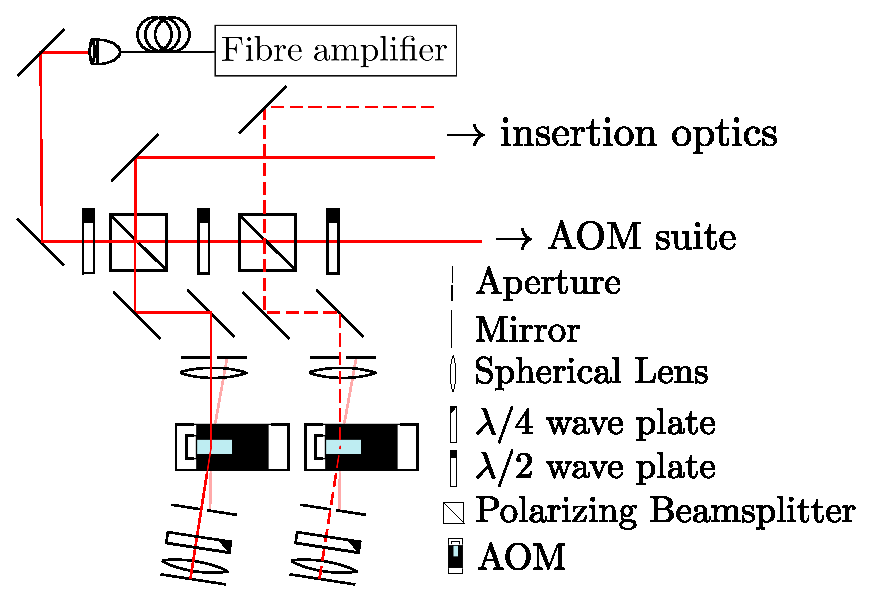
\includegraphics[width=\textwidth]{fig/lattice/distribution_optics}
		  {\fontsize{11}{13}
		  \begin{tabular}{l c c}
		  \hline\hline
		  Beam & Intensity & Detuning \\
		   & $(I_\textrm{sat})$ & ($\Gamma$) \\
		  \hline
		  Collimator &67& -5\\
		  Zeeman &92&-160 \\
		  MOT 1 &87 (Horz.)&-22 \\
		  		&110 (Vert.) & \\
		  Push &110&+3.3 \\
		  MOT 2 &37 (Horz.)& -33\\
		   &140,400 (Vert.)& \\
		  Imaging && \\
		  \hline
		  \end{tabular}}
	    \end{minipage}
	\end{figure}

	We had to align the collimator and Zeeman slower beams before the MOT could be build.
	Naturally, having set everything up perfectly the first time, the MOT was nowhere to be found.
	After some further tweaking, we obtained a visual signature of the MOT on the camera, a 1-2cm diameter smudge in the dark \footnote{We had to switch the room lights off to reduce scattered light in order to spot it.}.
	With some life breathed back into the old machine, it was time for a much larger operation.
	% We were pointing the old IR camera at the MOT chamber and looking for a change in brightness at approximately the middle of the trap, but saw nothing despite varying the alignment, polarization, and detuning of the beams while monitoring the video feed.
	% But there was no probe (photodiodes mostly useless as the chamber itself scattered more light than the MOT would) and no beam! The collimator and Zeeman slower beams also required alignment, including assembly of the beam-shaping and transport optics to either end of the table.
	% We coarsely aligned the collimator by maximizing the current on a faraday cup (the first in the middle of the Zeeman slower, the second at the end of the beamline after the MOT) with respect to the position of the two final mirrors before vacuum entry (unlike the BiQUIC machine, this beamline has three mirrors mounted in-vacuum and impossible to access for alignment).
	% The Zeeman slower was also aligned using faraday cups, but the rough alignment was first obtained by illuminating such a sensor located in the middle of the Zeeman slower (conveniently adjacent to a vacuum window) with a beam that was clipped down through an aperture.
	% The faraday cup at the end of the beamline (next to the Zeeman slower insertion window) provided the second point of constraint which we could use to ensure the laser beam was coaxial with the vacuum chamber.
	


\subsection{Vacuum build}

	
	The first stage of the build was to assemble the new science chamber.
	As we were waiting on delivery of the multichannel plates (MCPs) for the final detector, we assembled the second science chamber in order to get the low-velocity intense source (LVIS) operational in the interim.
	The first iteration of this build, prior to the addition of the MOT coils and optics, is shown in fig \ref{fig:first_build}.
	The large Kimball physics chamber features two 8" windows on the flat sides through which the vertical MOT beams and absorption imaging are inserted, and 4.5" windows for insertion of the dipole beams on the top and side opposite the LVIS.
	Several $\frac{1}{2}$" ports are used as feed-throughs for in-vacuum instruments (namely a channel electron multiplier \emph{a.k.a} channeltron for detecting ions produced by Penning ionization, a non-evaporative getter (NEG) to increase hydrogen adsorption and improve the vacuum, and a faraday cup on a rotation stage to measure the flux of metastable atoms into the chamber via the LVIS) or covered with windows for optical instruments such as a photodiode to measure fluorescence of the trap.
	The lower assembly includes four-way and six-way crosses (6" flanges each).
	The four-way cross featured a turbomolecular pump (opposite the point of view) which was backed by roughing pump.
	The six-way cross (at the bottom of the stack) featured a residual gas analyser (RGA), whose purpose is described below.
	The entire assembly was put together while supported by four jack stands (one on each flange of the six-way cross) on a pallet jack.
	The pallet jack could then be wheeled into position and raised to height, and then carefully docked with the back of the gate valve on the MOT.
	The apparatus also featured a discrete dynode elecron multiplier (manufactured by ETP) which was used in early attempts to detect atoms dropped from a magnetic trap, but later stopped working and was thus of no use as a diagnostic for the optical dipole trap.

	The `push' beam was aligned by maximizing the flux from the first MOT into the science chamber by measuring the current on a faraday cup.
	The sensor was positioned so that it could rotate into the beamline from its resting position out of any relevant optical paths.
	The current $I$ (in amps) gives an estimate of the order-of-magnitude flux $\phi_a$ of the atoms by the rule of thumb that $\phi_a\approx I/q$.
	This is an approximate method which is usually accurate to within a factor of 2-3 \cite{}, but easily suffices for diagnostic purposes.
	Once we obtained a signal that the push beam was reading a current of order 200pA, indicating a flux on the order of 10$^9$ \mhe atoms per second, we proceeded to assemble the rest of the vacuum system, shown in fig \ref{fig:underbelly}, and the MOT optics (section \ref{sec:new_optics}).
	The strategy was to assemble the MOT and absorption imaging systems to establish the magnetic and dipole traps, then use the ETP to optimize the dipole in the case we were still waiting on the MCP.
	The gate valve below the science chamber meant that we could close off the lower portion of the system and replace a single flange at the bottom of the 24" chamber when installing the MCP-DLD detector stack.
	Thus we would be able to perform the final upgrade without disturbing the MOT optics or breaking vacuum in the MOT chamber, which would be a significant advantage in that it would considerably simplify the necessary bake-out of the vacuum chamber, the subject of the next section.
	

	\begin{figure}
	  \begin{minipage}{0.55\textwidth} %4-8-16
	  \vspace{0pt}
			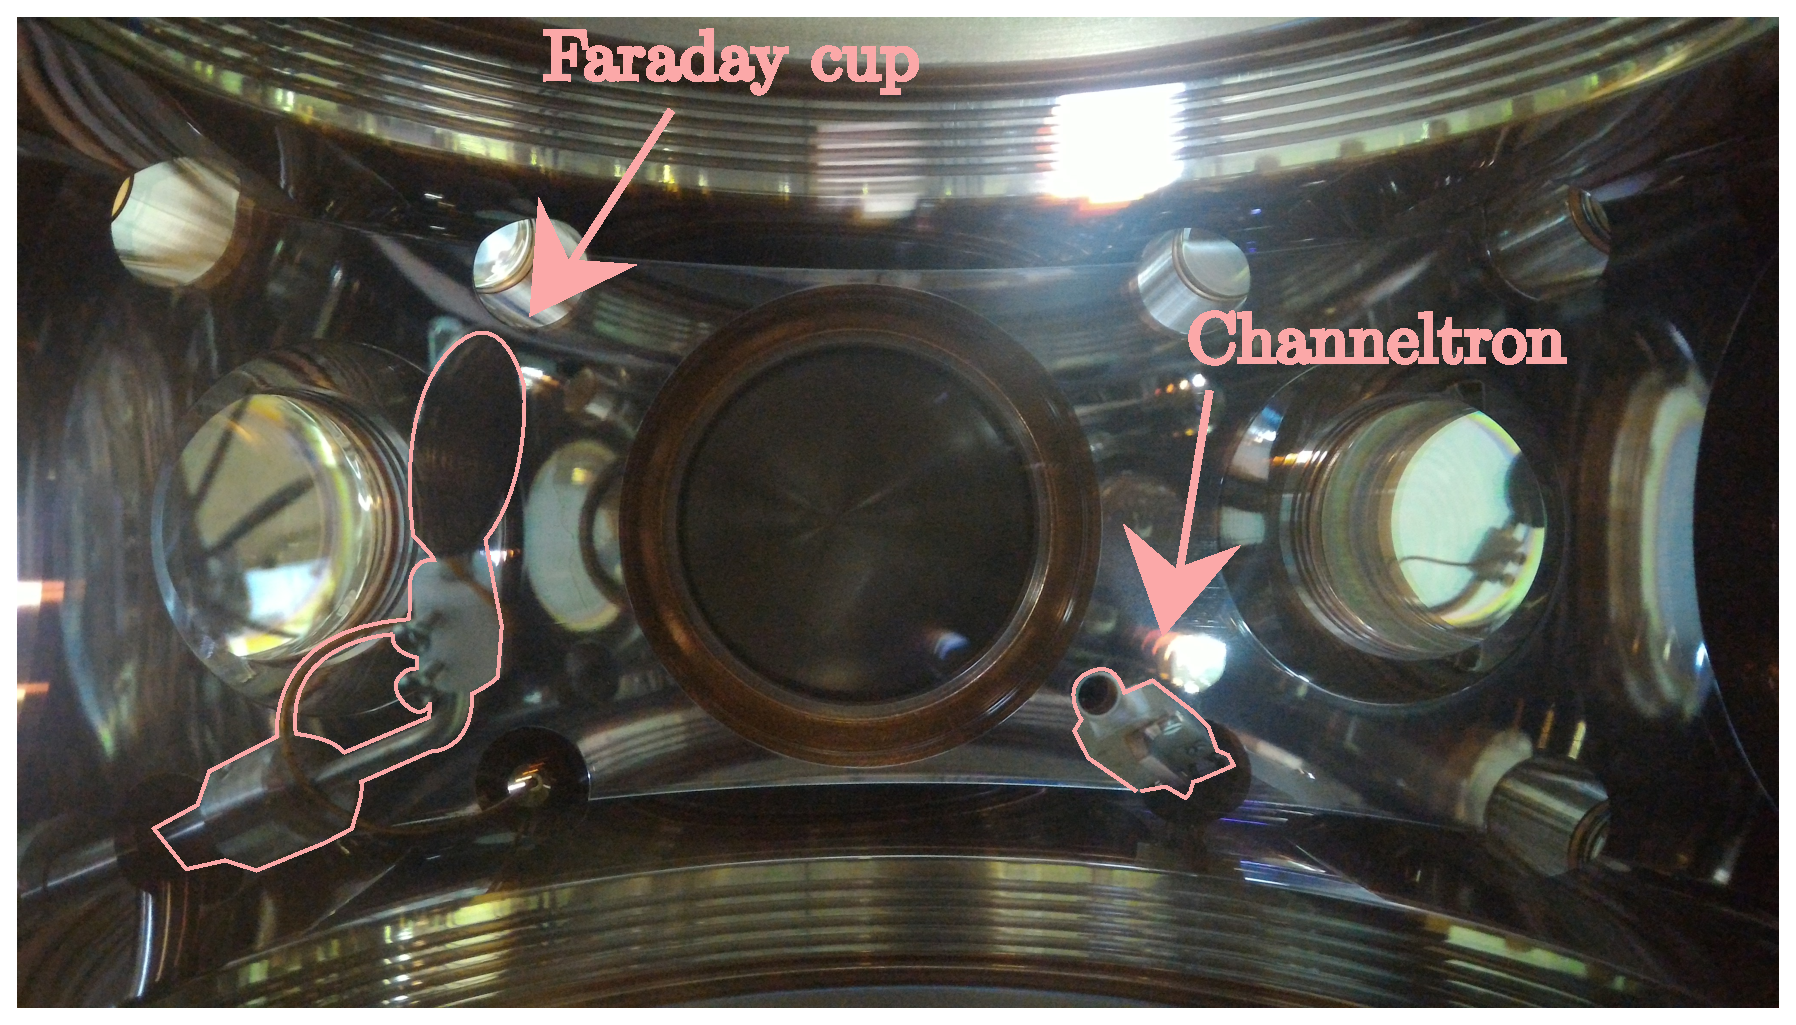
\includegraphics[width=\textwidth]{fig/lattice/science_chamber_internal}
		   {\begin{flushright}\caption{Initial build of the new science chamber.
	Right: The science chamber features several diagnostics (camera, Faraday cup, and channeltron) and a NEG for vacuum maintenance.
	Uses of the camera are discussed in sections below.
	A 6" gate valve separates the chamber from a temporary assembly underneath the table.
	Top: Internal view of the chamber, taken the preceding day (after which the channeltron was moved to make room for the mounting plate, see below).}\end{flushright}\label{fig:first_build}}
	  \end{minipage}
	  \hfill
	  \begin{minipage}{0.45\textwidth}
	  \vspace{0pt}
		\includegraphics[width=\textwidth]{fig/lattice/science_chamber_profile}  % 5-8-16
	  \end{minipage}
	\end{figure}


	
	
	\begin{figure}
			\centering
		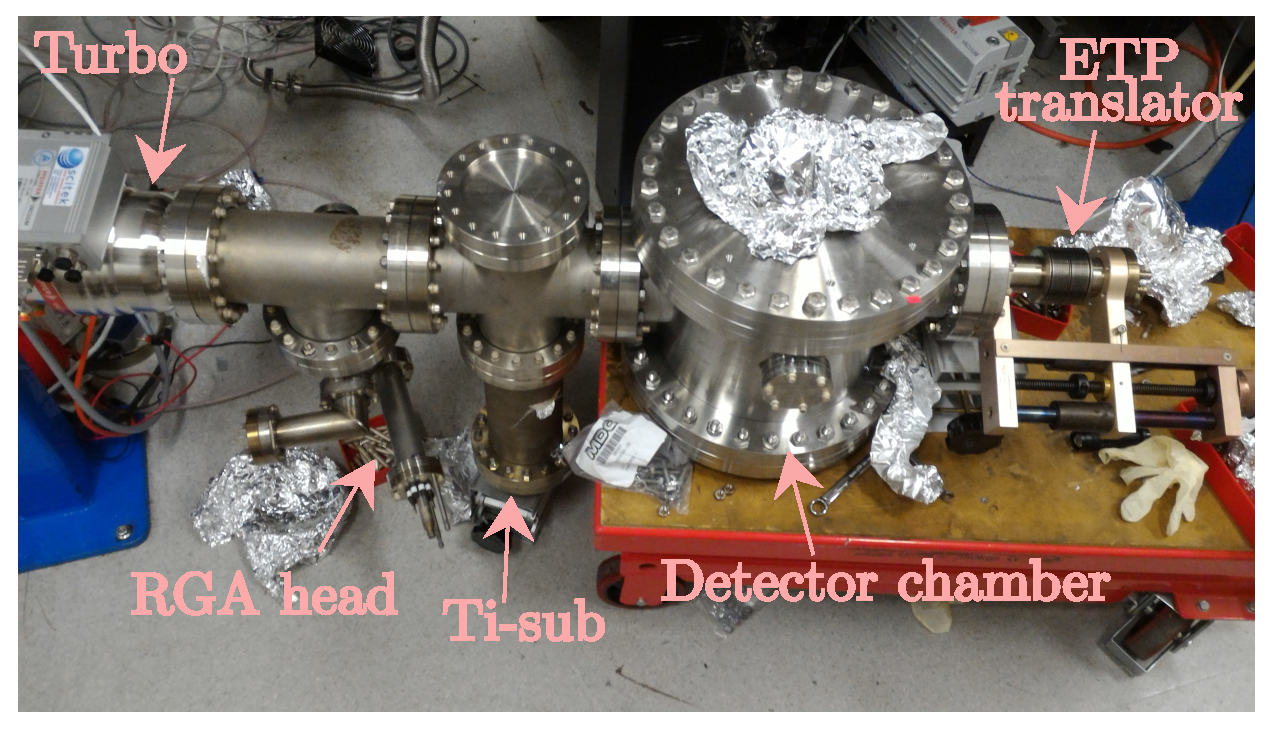
\includegraphics[width=\textwidth]{fig/lattice/detector_level.eps} %15-9-16
		\includegraphics[width=\textwidth]{fig/lattice/full_assembly_20160915} %15-9-16
			\caption{The leviathan-like underbelly of the science chamber resting after assembly on the mobile pallet jack and a smaller hand jack to support the TiSub.
		 The science chamber was re-mounted with an intermediate gate valve and then wheeled into place.
		The assembly was stabilized on the blank flange at the bottom of the {24"}-diameter detector chamber, and by being \emph{really} heavy.}
	\label{fig:underbelly}
	\end{figure}

	


	
	\subsubsection{Improving vacuum conditions}

		As mentioned in chapter \ref{chap:exp}, the viability of cold-atom experiments depends on having a good quality vacuum.
		Any background gas molecules will typically have thermal velocities of several hundred m/s, with kinetic energies many orders of magnitude larger than the traps.
		Thus an overabundance of background can dramatically reduce the lifetime of magnetic and dipole traps such that evaporative cooling to degeneracy may be impossible.
		In the case of helium, there is the added issue of the small atomic mass and possibility of Penning ionization (even in low-momentum collisions) which only exacerbare the issue.
		This lab does not maintain cleanroom conditions in the entire room, so even though care was taken to cover components in new foil when they were not being handled, some environmental pollution would be inevitable.
		Water a common contaminant, but handling errors can also be a problem, and dust or aerosols can accumulate invisibly on the steel surface
		All of these contaminants become problems when pumping down to vacuum as the pressure rapidly drops below the vapor pressure of many chemicals that may be stable in atmospheric conditions.
	
		These surface contaminants may outgas slowly (or be comparatively large) and present as persistent `virtual leaks' in the chamber.
		The standard remedy is to wrap the machine in highly resistive wires insulated with fibreglass, cover it with aluminium foil to keep heat in, and baking the entire apparatus at up to 150 degrees celsius for several days.
		The chemical makeup of gaseous contaminants can be determined using a residual gas analyser (RGA) which are essentially compact mass spectrometers.
		The initial evacuation of the chamber by connecting the turbomolecular pumps was enough to observe a magnetic trap, but would be insufficient to make further progress (see fig. \ref{fig:lifetime}).
		Figure \ref{fig:RGA} shows the partial-pressure contributions of gaseous contaminants before the first bake.





		% The interior of the vacuum chamber can be contaminated during the build process.
		% We typically wore nitrile gloves when working on the build, but they can pick up residue when touching (intentionally or not) other surfaces.
		% Where it was necessary to clean internal surfaces, we usually used ethanol because it is very volatile, but it may also have trace impurities and occasionally we noticed a residue was left behind when it made contact with the gloves, for instance through the lens tissues used for wiping down surfaces.
	
		% Of course, the tissues themselves can leave traces despite being `lint-free'.
	

		The higher temperature during the bake increases the outgassing rate and can even liberate some contaminants from the surface, allowing them to be pumped out by the turbomolecular pumps.
		In this process one typically observes a sharp rise in pressure as the chamber heats and the contaminants vaporise, and then a decrease to a lower steady-state pressure as the contaminants cease outgassing and the remnants are evacuated.
		Once the pressure stabilizes, the heater tapes can be turned off, and as the apparatus cools the pressure will settle to a more preferable level.
		An example of this procedure is illustrated in Fig.	\ref{fig:bakeouts}.
		
		Even after baking, the pressure may not be low enough to permit long-lived traps.
		Hydrogen leaching from the surface of the steel chamber can be significant, and even permeate the steel on long enough timescales.
		One means of addressing this is with a titanium sublimation pump (TiSub).
		This is not a pump \emph{per se} but rather a titanium filament.
		A pulsed current of $\approx5A$ (duty cycle approximately 30 seconds on, 60 seconds off) heats the filament and causes titanium to sublimate off the surface and adsorb onto the interior surface of the steel vacuum chamber.
		Hydrogen adsorbs to the titanium surface but not to steel, and so after some applications the pressure trends further down.
		% An example of this process is shown in Fig.	\ref{fig:bakeouts}.
		% During the `on' phase of the TiSub the pressure spikes (sometimes by a few orders of magnitude) and then relaxes again in the `off' phase as the sublimated metal settles on the steel or is pumped away.
	
		% The short duty cycle means that the relaxation pressure is not necessarily a good indicator of the long-term pressure but it is common to see the relaxation pressure decreasing, and when this reaches a steady state the process is terminated.
	
		

	\begin{figure}
		% 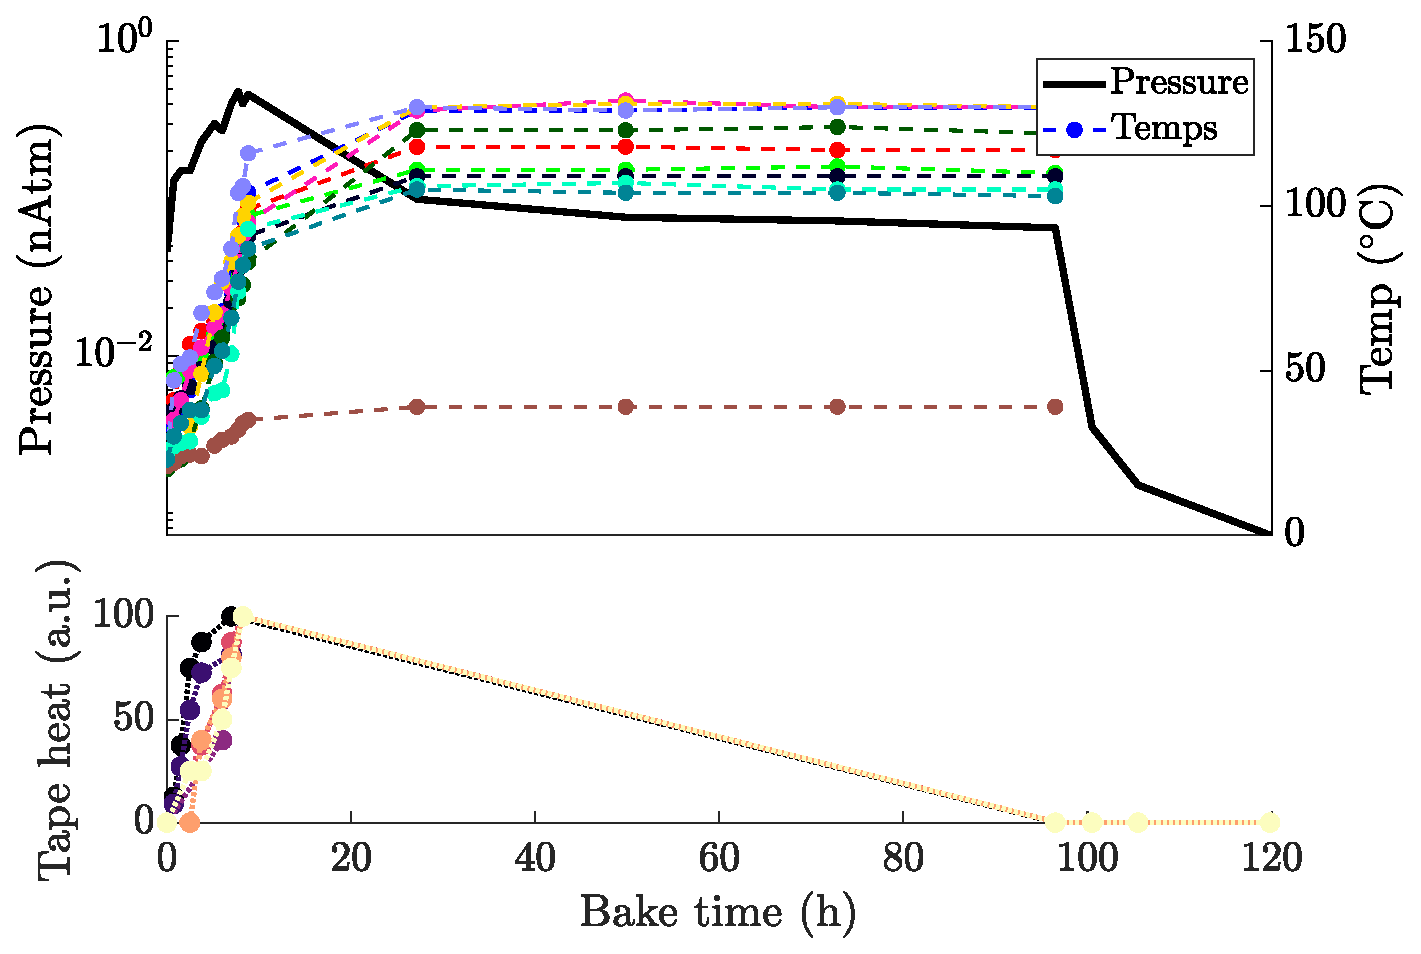
\includegraphics[width=0.5\textwidth]{fig/lattice/mid_december_bake_chart}
		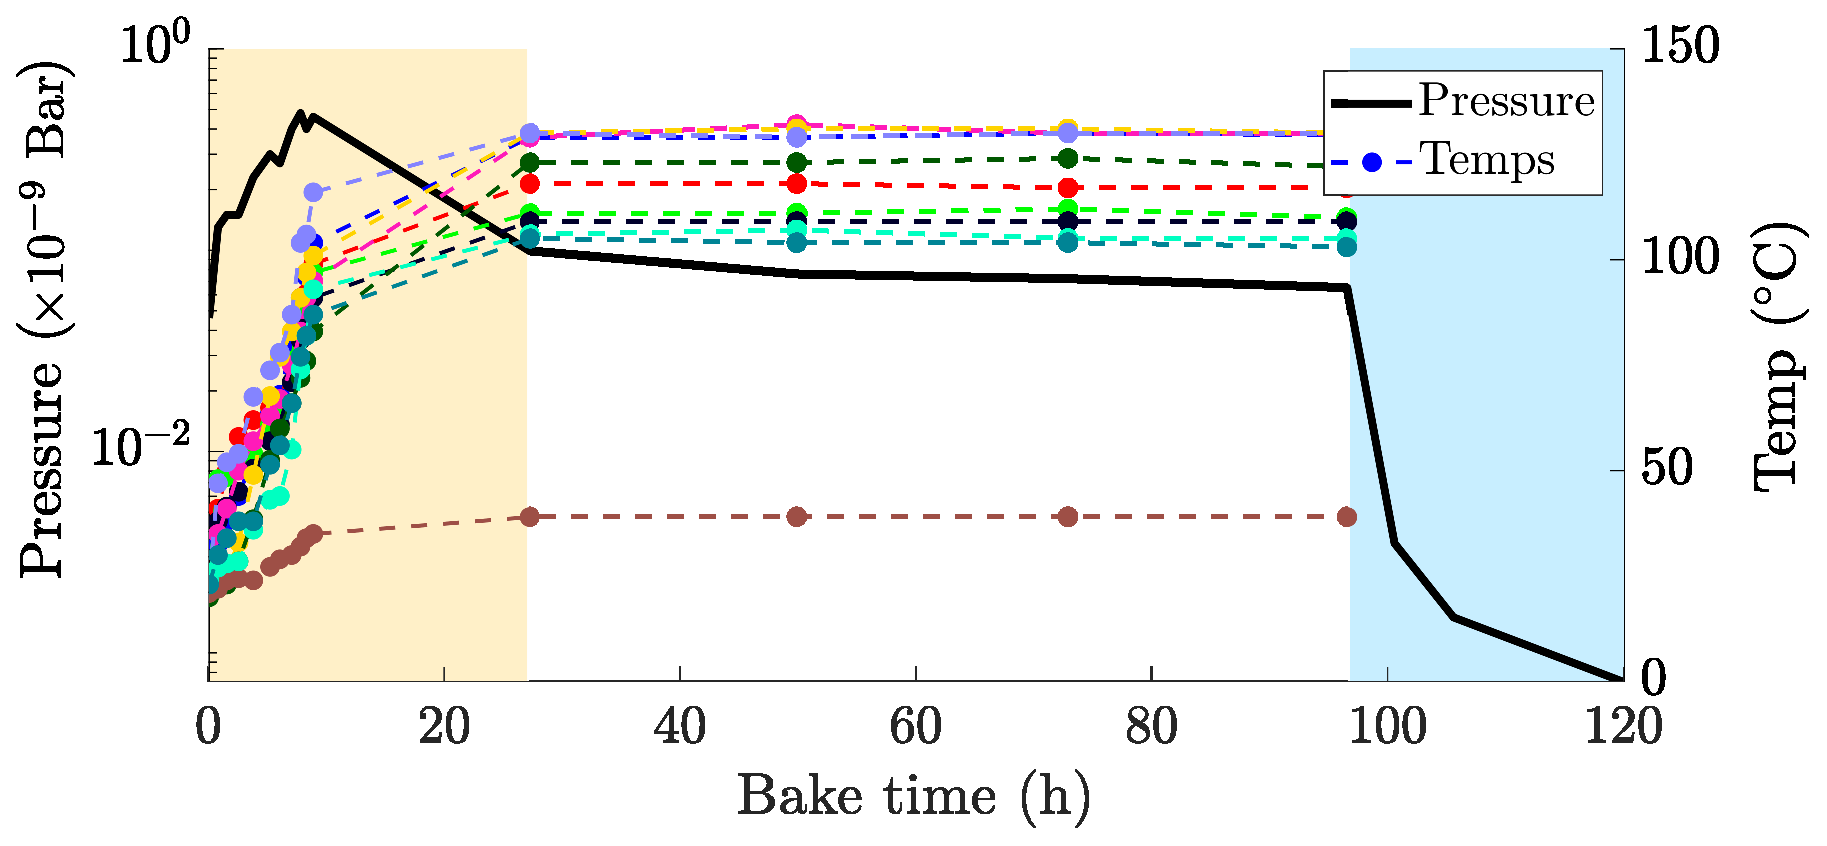
\includegraphics[width=\textwidth]{fig/lattice/bake_record.eps}
		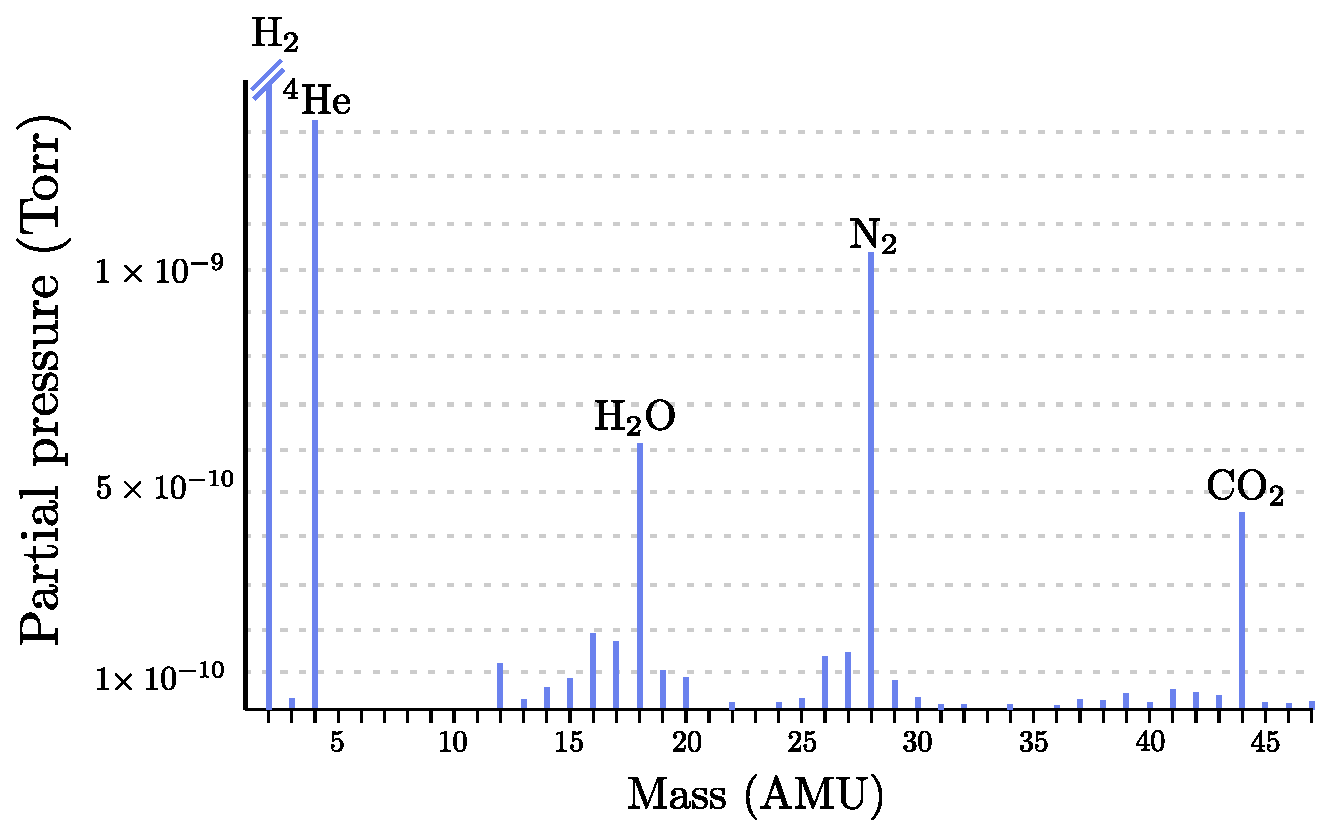
\includegraphics[width=\textwidth]{fig/lattice/RGA_pre_bake_nice}
		\caption{Top: The temperature measured by several thermocouples taped to the surface of the vacuum chamber (dots with dashed lines) and the pressure readout from the ion gauge on the science chamber during a bake.
		The heater tapes are supplied with current from variable voltage sources (variacs) which are turned up gradually to ensure even heating when starting the bake (orange region).
		After the tapes are switched off and the insulating foil opened, the steel quickly cools and the vacuum pressure stabilizes (blue region).
		The lower (brown) temperature curve was measured with a thermocouple on the flange connecting the 6" T-piece to the turbo (see fig \ref{fig:underbelly}) which was kept cool to avoid excessive heating of the turbo itself. 
		Lines in this figure are to guide the eye, individual measurements are denoted by the solid points.
		Bottom:
		Gas concentrations before the first bake as measured using the residual gas analyser (RGA). \todo{
		A before/after graph would be nice, but I don't know if we have one...}
		}
		% 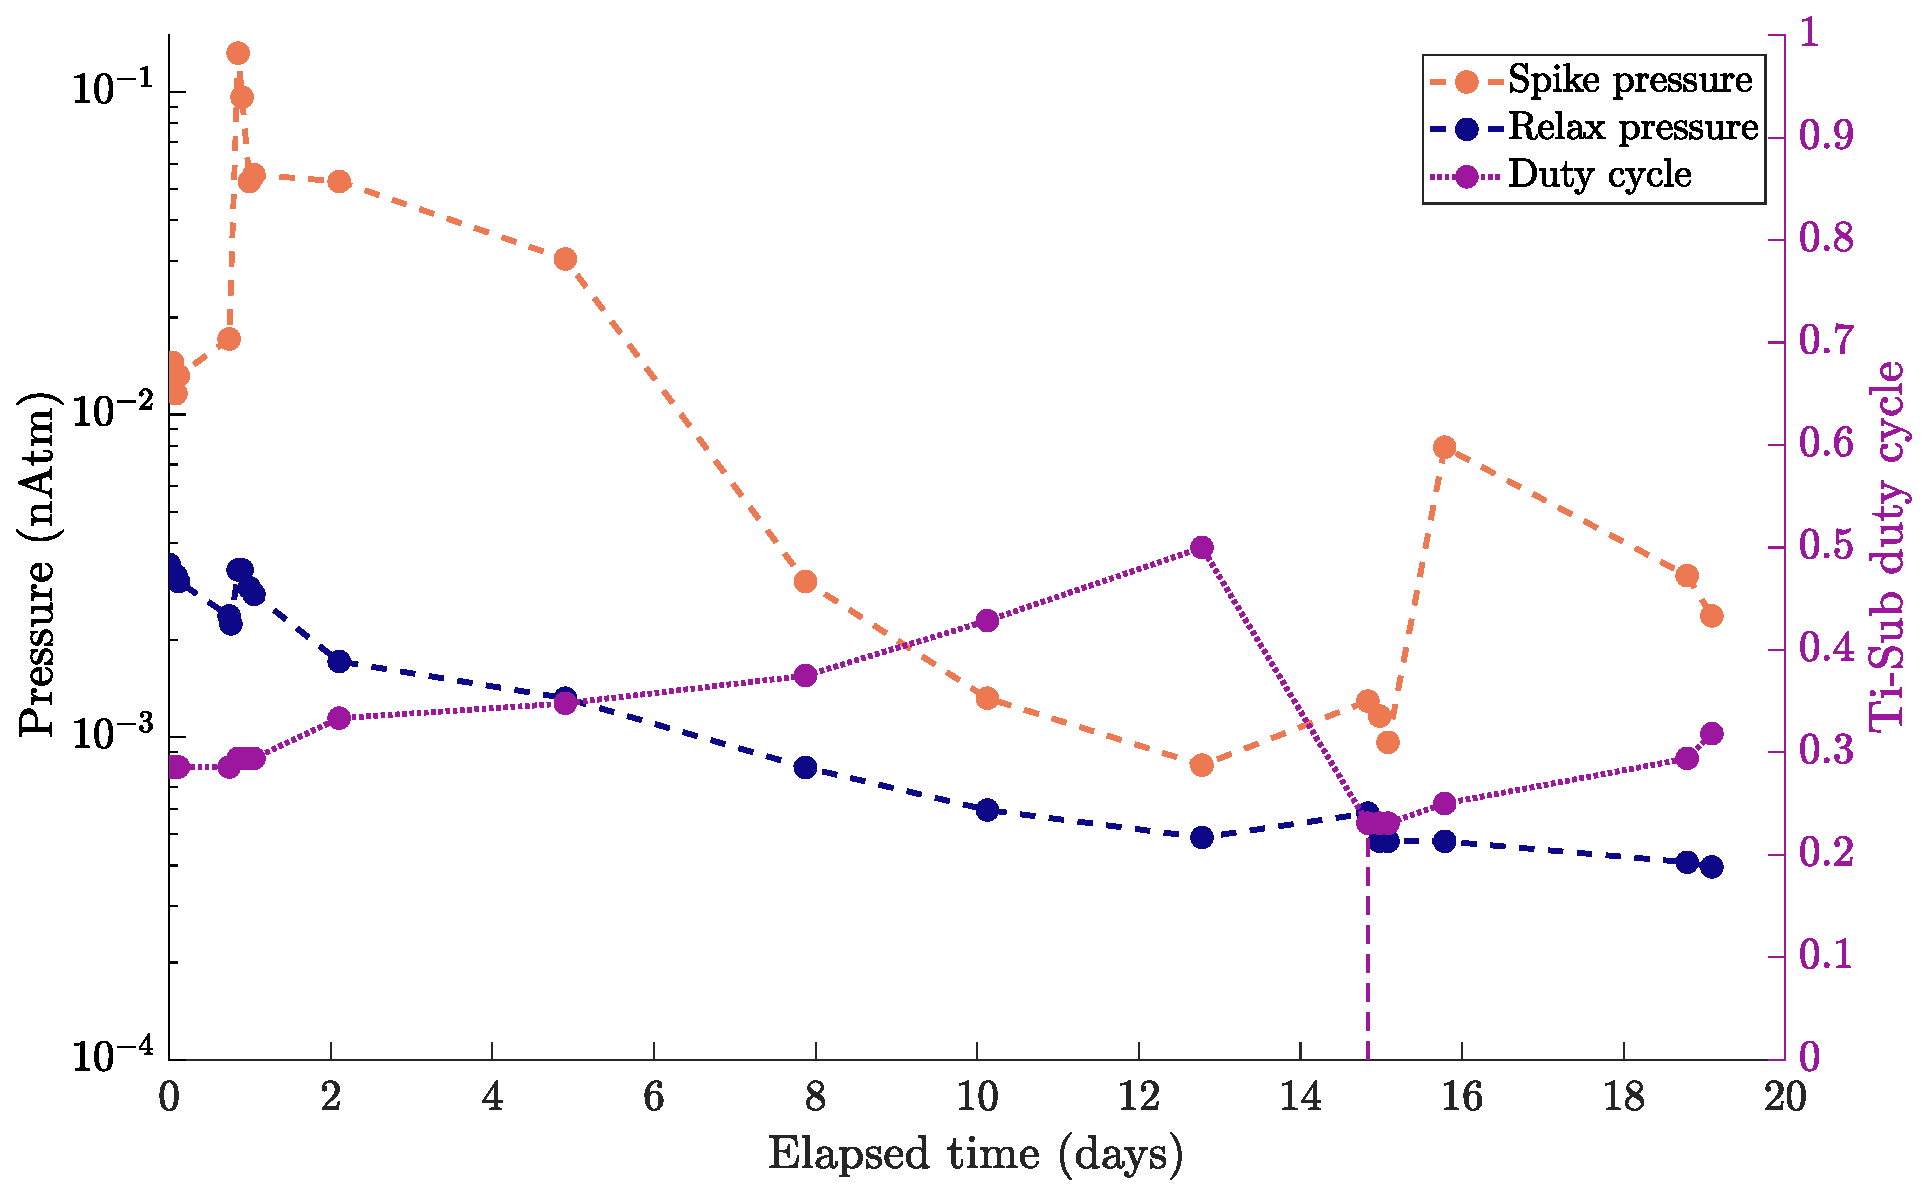
\includegraphics[width=0.9\textwidth]{fig/lattice/tisub_record}
		\label{fig:bakeouts}
		\end{figure}
	% Bottom: The application of a TiSub driving down residual hydrogen pressure over the course of several runs.
	% The pressure peaks as surface contaminants volatilize off the filament.
	% As the spike pressure diminished despite increasing the active duty cycle, we switched to a new filament on day 15 and found better sublimation rates at very low duty cycle.
			
	% Probably remove the TiSub graph.
	% Variac graph isn't useful - just shade/mark regions on top plot to show ramp up and switch off.
	% The temperatures are also not particularly meaningful and their large range deserves some comment.
	% What was the lower one, in particular?}

		A further pressure reduction can be obtained by `getters' which operate in a variety of ways (a TiSub is a kind of hydrogen getter).
		In our machine we used a non-evaporative getter (NEG) in the science chamber.
		The NEG has a highly porous active area which adsorbs hydrogen very strongly.
		This means that they tend to carry in a lot of contaminants and have little remaining active area when first pumping down.
		We clear the surface of the NEG by passing up to 5A of current through it.
	Again, the pressure spikes and eventually relaxes up to an hour later, when the current is switched off.
		As shown in fig \ref{fig:bakeouts}, chamber bakes can improve the chamber pressure by up to three orders of magnitude.
	Afterwards, the TiSub can improve the pressure by a factor of five to ten, and the NEG by a factor of two to five.
		
		
		% Over the course of the vacuum build (and in the course of subsequent renovations, accidents, and so on) we baked the experiment several times.
		% The baking process itself requires little attention but means no work can be done in the vacuum.
		% Plus, there is considerable overhead in disassembling optics, wrapping the machine up, babysitting it over the first day, unwrapping it, and (by far the worst) reassembling and realigning the optics afterwards.
		% All this adds up to a general necessity to avoid breaking vacuum unless absolutely necessary.
		The payoff for this multi-stage procedure is the enormous reduction in background pressure that permits long-lived magnetic and (purely) optical traps.
	
		The lifetime can be quantified by any means that provides a reasonable proxy of the trapped population (the quantity of concern is the relative population at some time later), such as in Fig.	\ref{fig:lifetime}.
		Currently the machine operates at a background pressure of at most 3$\times10^{-11}$ mTorr \cite{Abbas21}.
	






\subsection{MOT and magnetic trap}
\label{sec:new_optics}

	\begin{figure}
		\includegraphics[width=\textwidth]{fig/lattice/science_chamber_oblique} %4-8-16
		\includegraphics[width=\textwidth]{fig/lattice/science_chamber_optics} %3-5-17
		\caption{The first iteration of the science chamber (in August 2016)  illustrating the coordinate axes used in the lab and the mounting surfaces for the magnetic coils (one of the Anti-Helmholtz (AH) coils was mounted on the back face of the large Kimball chamber). 
		The channeltron is visible on the lower right of the chamber (top), but was moved the next day to make room for the MOT mirror in a similar location in the later image.
		This configuration was used to test vacuum viability and align the LVIS.
		Once the new optic-mounting platform had ben constructed by technician Ross Tranter, we could install the MOT optics (bottom, mounting plate in lower-left quadrant).
		The MOT and imaging beam trajectories are marked, along with the direction of propagation of the LVIS.
		The faraday cup and NEG are still installed in the lower picture, but the NEG is obscured by the chamber.}
		\label{fig:MOT_optics}
	\end{figure}
	% 1.7e8 atoms loaded at 2.5mK in 1 second, as measured using saturated fluro on an InGaAs PD [26]
	With a good, clean, vacuum and ample optical bench space around the science chamber, the optical components could finally be installed.
	Figure \ref{fig:MOT_optics} shows the enclosing construction around the science chamber that supports a MOT, magnetic trap, and absorption imaging.
	First, the magnetic coils \todo{Get coil specs} were mounted on the windows to create the anti-Helmoltz field (with axis of symmetry along $x$, parallel to the Zeeman slower) and a bias field directed along the $y$ axis, back along the LVIS.
	The diagonal MOT beams enter through the 2$\frac{3}{4}$" widows on the 45$^\circ$ ports.
	\ref{fig:MOT_optics}.
	We used the channeltron as a sensor for the presence of a MOT during initial alignment.
	A poorly-aligned MOT (or one with unfavourably set beam parameters) would not have been easily visible by camera or photodiode, but the increase in Penning ionization rate would in principle be controllable by blocking a MOT beam and hence provide a fast diagnostic.
	The MOT itself could only be constructed after installing a mounting plate around the base of the vacuum chamber, which was installed after baking the entire new assembly.
	


	\begin{figure}
		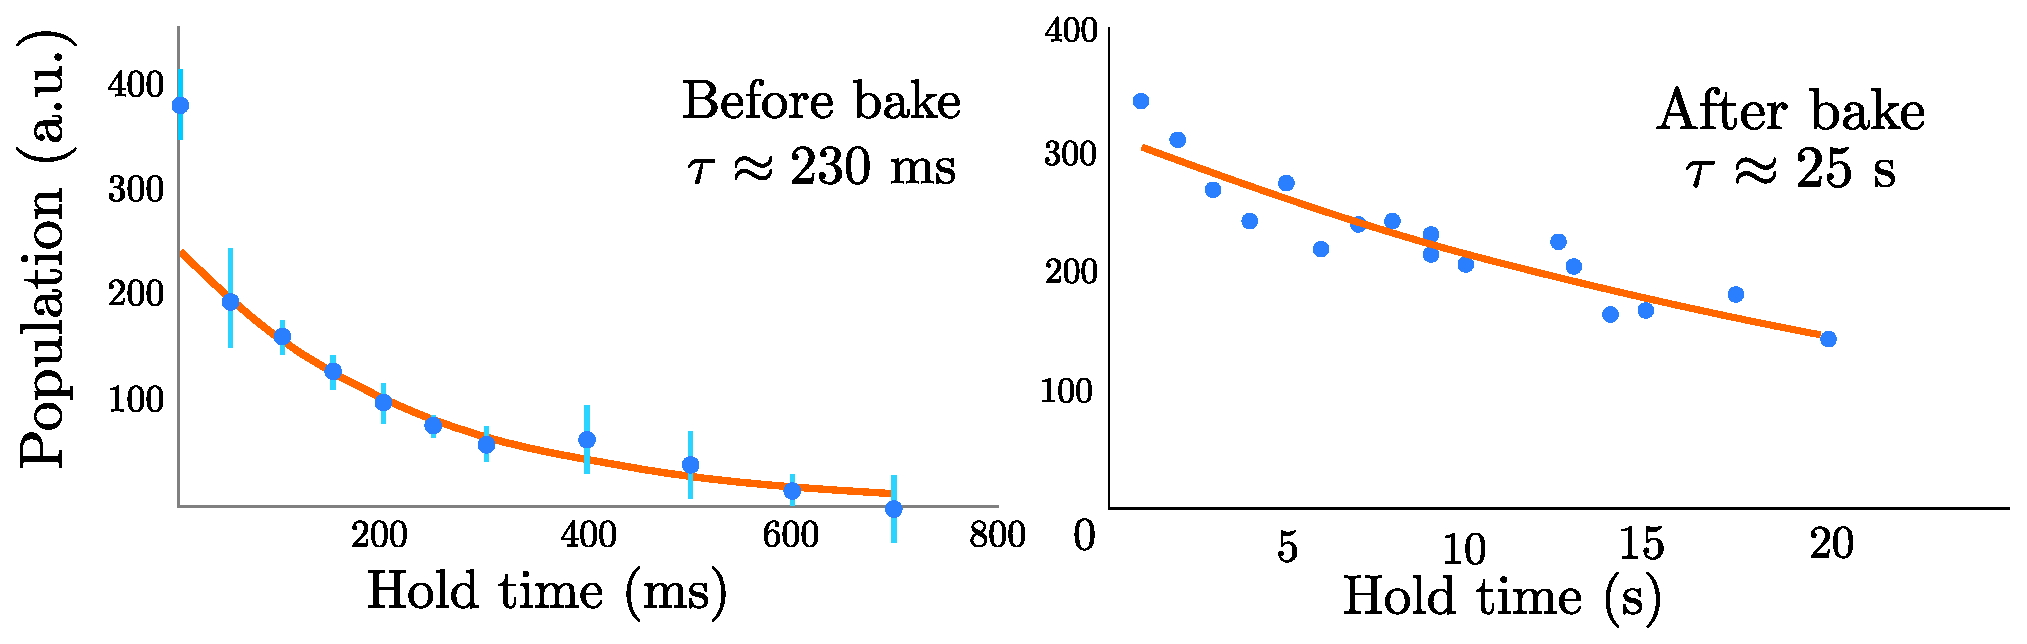
\includegraphics[width=\textwidth]{fig/lattice/trap_lifetimes}
		\caption{Magnetic trap lifetime measurements using before and after baking the new vacuum system. 
		The uncalibrated measurements only show the relative population, due to the measurement method described in section \ref{sec:abs_img}.
		Data points in the left plot are taken from averages of three shots, points on the right plot are single shots.
		The lines in both graphs are exponential fits.}
		\label{fig:lifetime}
	\end{figure}


\subsubsection{Absorption imaging}
\label{sec:abs_img}
		
	Alignment of the dipole trap was eventually made possible by absorption imaging.
	This imaging system also provides access to measurements of the temperature, density, atom number, and thus phase space density of a trapped cloud.
	This system is preferred over the MCP-DLD for imaging MOTs and magnetic traps because 
	the clouds can be so wide on the detector that it is impossible to accurately determine the width, thus temperature, of the cloud.
	The analysis can be made more difficult by the potential saturation of the detector at large fluxes.
	A final, albeit lesser, concern is that MOTs and magnetic traps contain thousands of times as many atoms than remain after condensation and so they would shorten the detector's lifespan.
	

	\begin{figure}
	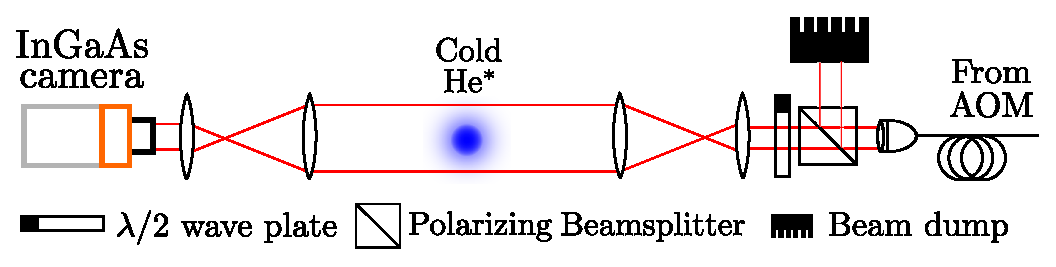
\includegraphics[width=\textwidth]{fig/lattice/abs_img}
	\begin{minipage}{0.45\textwidth}
	\vspace{0pt}
		\caption{ Above: Schematic of the absorption setup as described in the text.
		Adjacent: 
		Example image of the MOT.
		In practise the shot noise on the camera can be significant, and so for visual inspection a smoothing kernel is applied.
		Because of the issues in the text, it is nontrivial to make meaningful inferences about trap properties from in-trap images like these.}
		\label{fig:abs_img}
		\end{minipage}
		\hfill
		\begin{minipage}{0.54\textwidth}
	    \vspace{0pt}
	    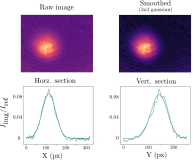
\includegraphics[width=\textwidth]{fig/lattice/20170606_CMOT_img}
	    \end{minipage}
	\end{figure}
	% Shown instead are sections of a two-dimensional Gaussian fit to characterize the trap size and central density, both of which can be used as measures to optimize against.}
	% Initial alignment of the imaging beam was facilitated by the use of a camera mounted above the science chamber (as visible in Fig \ref{fig:science_chamber} \todo{Broken ref, maybe 'as shown in previous figure'}, with the same field of view).
	% The intention was to take an image with the camera simultaneously with a pulse of light down the imaging line and observe the cloud fluorescing \todo{This isn't clear}.
	% It turns out that with a longer exposure time after switching on the light, one can observe this 'cold-atom comet' as the atoms are pushed along by the radiative force of the beam, fluorescing along the way \com{Are you sure this is what it is showing?  Looks like it's at the wrong angle, plus the streaking seems to extend into the window, so I'd guess it could be pixel streaking.}.
	% Lower right: 

	A simple description of absorption imaging is that one `takes a photo of the shadow of the atoms' by illuminating the sample with a collimated laser beam, and then projecting the beam onto a camera (Xenics Bobcat, as above).
	
	Detailed discussions of the physical principles and implementations of this technique are presented in \cite{MakingProbingUnderstanding,TychkovThesis}.
	Here we present a simple picture.
	A laser tuned close to resonance with the atomic sample is coupled via optic fibre to the absorption imaging setup.
	The light passes through a polarizing beam splitter and then a half-wave plate to fix then set the polarization, which is useful when imaging in the presence of a bias field\footnote{And indeed the earth's field, which was later found to be strong enough to suppress Penning ionization sufficiently to achieve condensation \cite{Abbas21}.}.
	The beam is then magnified by a 4:1 telescope to a $\approx1$ cm collimated waist and directed at the atomic sample through the vacuum windows.
	The electric field on the exit side of the cloud will have been attenuated by a factor $Ae^{i\phi}$, where the attenuation factor $A=\exp(-\frac{\tilde{n}\sigma_0}{2}\frac{1}{1+\delta^2})$ depends on the column density  $\tilde{n} = \int n(x) dx$ (integrated along the beam axis), the detuning in (half-linewidths) $\delta=2(\omega-\omega_0)/\Gamma$, and the absorption cross-section which is $3\sigma_0\lambda^2/2\pi$ in the two-level approximation \cite{MakingProbingUnderstanding}.
	The phase $\phi$ also depends on the atomic density and detuning from resonance, and is in principle useful for techniques like phase contrast imaging, but is not presently used in our experiment.

	The camera records an image during the application of the laser light and a second image of identical exposure time after a f{$\approx$10ms delay}\footnote{We found it helpful to ensure that the AOM switched off in the meantime as well, and turned back on for the same cycle time for the second measurement.
	The AOMs can exhibit slow rise-times to their steady state pointing and efficiency due to disippation of heat into the crystal from the RF drive.
	This was measurable as differences in the light intensity between subsequent images if the AOM was left on between exposures.}
	By this point the atoms have scattered many photons and left the laser path.
	The second image is used as a reference to compute the integrated absorption at each pixel.
	A light-free image can be used as a `darkfield' to compensate for the camera's inherent noise profile.
	The ratio of (calibrated) pixel intensities in the presence of atoms $I_\textrm{abs}$ to the reference image without atoms $I_\textrm{ref}$ then provides a measure of the (squared) transmission coefficient
	\begin{equation}
	A^2(x,y)=\frac{I_\textrm{abs}-I_\textrm{dark}}{I_\textrm{ref}-I_\textrm{dark}}.
	\end{equation}
	The 2D absorption profile can be fitted for purposes of further quantitative analysis. 
	Imaging in-trap is certainly possible and useful for optimizing performance, but it introduces the complication of a spatially-varying magnetic field.
	This means that the transmission coefficient varies due to the Zeeman shift around the trap.
	However, the initial imaging setup had too large a magnification to image the far-field density distribution which is necessary for thermometry.
	This design was shaped by the objective to load atoms into the dipole trap by using absorption imaging as the diagnostic, hence the magnification was chosen such that the MOT would almost fill the frame of the camera sensor.
	Therefore thermometry was not performed using this technique. 
	This was a shortcoming of the first design which was later remedied by upgrading the magnetic coils (see below), thus producing a more tightly-confining field and thus a denser trap.
	For detection and analysis of clouds released from a dipole trap, the lab currently uses the pulses of current across the MCP plates to infer the time-of-flight of atomic detection events \cite{Abbas21}.
	Calibration of the DLD for reconstruction of spatial information is currently underway.

	We could still perform (approximate) population measurements by fitting a Gaussian profile to the images.
	Unforunately this was not adequately sensitive to measure the lifetime of the magnetic trap.
	After a short decay time it became impossible to get a good fit or even to see the cloud by eye in the absorption images, and thus the long-time behaviour was inaccessible.
	Instead, we released atoms by turning off the magnetic trap and used the number of detection events from the ETP electron multiplier (passed through a NIM crate including a constant fraction discriminator, amplifier, and pulse rate counter which passed into the LabView software) as a proxy for the population.
	The lifetime could then be obtained by an exponential fit to the measured populations over time.
	Measurements of the magnetic trap lifetime before and after the chamber bake are shown in \ref{fig:lifetime}


	
	

\subsection{Dipole trap}
	While the main chamber was unworkable during bakeouts, construction could continue on other components of the machine, including the control and distribution systems for the optical dipole beams.
	A 1550nm diode laser source seeds a 30W fibre amplifier with a linewidth of $\approx100$ kHz.
	The high-power beam is split into two AOM arms in a similar manner to the cooling optics described above.
	This configuration is illustrated  in Fig.	\ref{fig:dipole_optics}.
	% Because of the high power and stability demands, the optics were mounted on sturdier posts.
	
	To mitigate against misalignment of the dipole beams, which would eventually need to be overlapped in the focal region within less than 100 $\mu$m, we coupled light from the generation optics to the shaping optics via high-power NKT Photonics photonic crystal fibres to ensure the downstream optics are independent of the alignment upstream.
	Each AOM was driven at a fixed frequency by an amplified voltage-controlled oscillator, but the drive power was set in closed-loop configuration (as opposed to the cooling optics).
	The voltage from a post-fibre photodiode was returned to a PID controller whose set point was determined by an arbitrary waveform generator, which was pre-loaded with user defined waveforms and triggered by the main DAQ system.
	After losses in AOM transmission efficiency and fibre coupling losses, the maximum achievable (total) efficiency of each arm was about 25\% (defined as the ratio of power delivered into the chamber over the input power to the respective AOM).
	While I was working in the lab, the beam powers were roughly equal, but in the interim the dipole system has been redesigned, and is discussed in \cite{Abbas21}.
	% The lenses were mounted on rails which had been bolted the table.
	% Millimeter markings on the side of the rail assisted in testing reproducible optical configurations and almost eliminating a degree of freedom of error.
	% In any case, routine realignment is periodically necessary and so the separation of functions is essential \todo{What does this mean/is it necessary?}.
	% Further, operating the AOMs with such high power heats the crystals and modifies the refractive index and the pointing of the outgoing beam (also the efficiency but not to a significant degree) \todo{How was this mitigated?  The mitigation you refer to in the next sentence is a completely separate issue!}.
	
	
	\begin{figure}
		\centering
		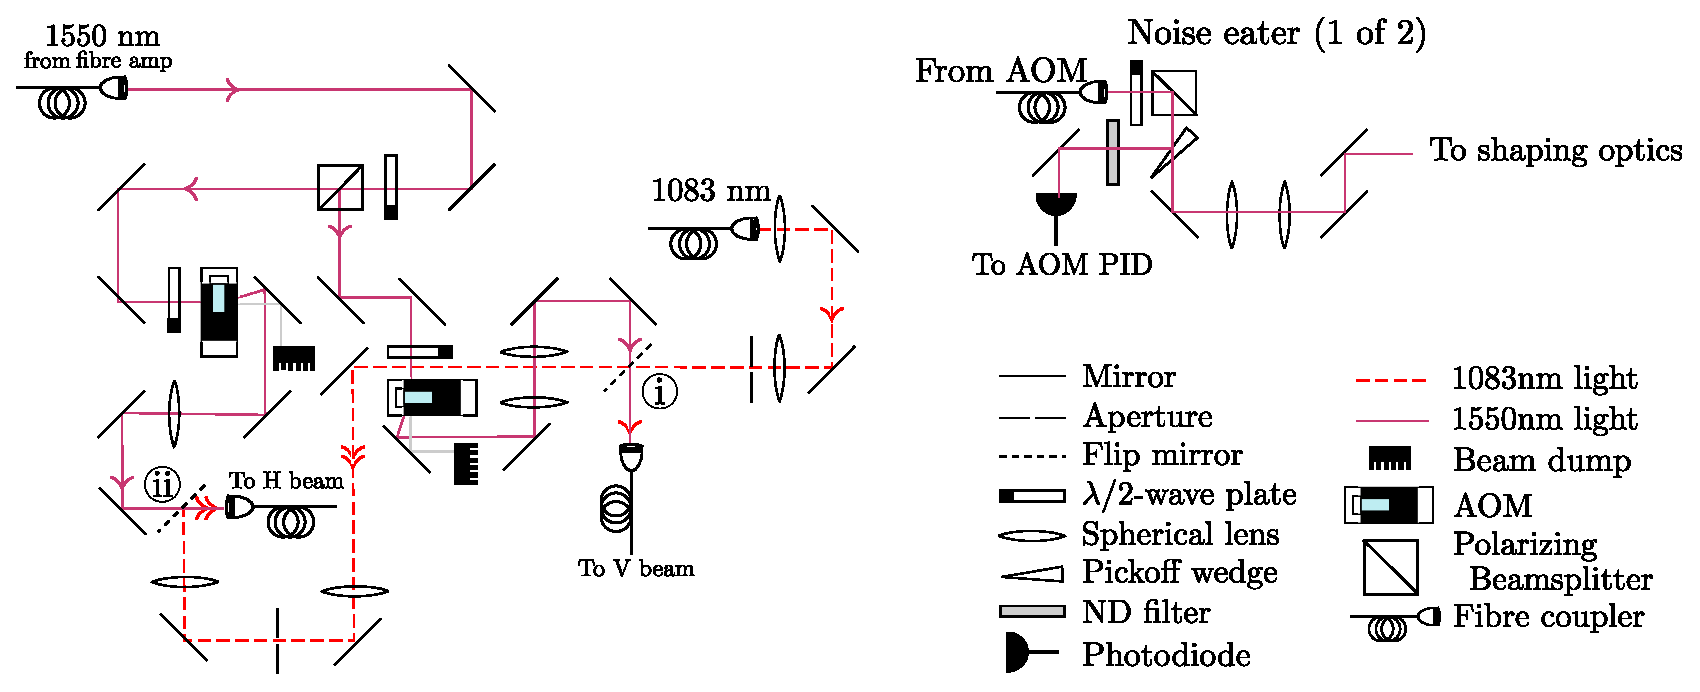
\includegraphics[width=\textwidth]{fig/lattice/dipole_optics}
		\caption{Schematic of the 1550nm optics used to generate and control the the dipole trap beams in the lattice machine.
		The AOMs are used for amplitude control and fast switching.
		They are driven by dedicated PID controls set in configurable sequences with the arbitrary-waveform generators.
		The beams then focus into an optical fibre which transports the beam to the shaping optics (example on top right).
		Initial alignment of the dipole beams is achieved one beam at a time by inserting one of the removable mirrors (marked (i) and (ii)) and coupling resonant 1083nm light into the fibre.}
		\label{fig:dipole_optics}
	\end{figure}
	

	It is generally desirable to operate far-red-detuned dipole traps at very high intensities to create deeper traps (recall the ground-state shift scales with the intensity $I$, c.f.
	chapter 1).
	Deeper optical dipole traps can contain higher phase-space density at a given temperature by virtue of trapping over a larger range of particle momenta, and so greater laser intensity is generally a good thing.
	It is true that spontaneous off-resonant scattering rates increase (approximately linearly) with intensity, but this could be remedied by detuning further (the scattering rate falls off with $\Delta^2$).
	Therefore one can obtain better loading efficiencies by using brighter beams.
	The purpose of the shaping optics are thus to shape the profile of the beam such that it reaches a tight focus.
	In order to achieve this, given the non-collimated laser profile emitted from the fibres, we first had to determine the profile of the beam, and then determine an arrangement of lenses to shape the beam to a tight focus at the desired trap location.
	The procedure we used to construct the shaping and insertion optics are discussed here.
	We aligned the beam output from the fibre parallel to a 1m-long rail which would be used to mount the lenses.
	We measured the profiles (at low power) by taking images with an InGaAs camera and fitting the output images with 2D gaussian profiles (The camera was a  Xenics bobcat, 256x320 resolution, 20$\mu$m pixel pitch, is also used for absorption imaging).
	A constrained two-dimensional Gaussian fit yields the waists $\sigma_x$ and $\sigma_y$ along the frame axes.
	
	 % (where the numerical aperture is limited to $\mathcal{O}(.02)$ by i) the placement of the final lens outside the vacuum chamber some 50cm from the target focus and ii) the use of 1" optics)	
	% \todo{This needs some rephrasing.
	% a) it's not clear we are diffraction-limited, b) the NA is mostly limited because the lenses are so far from the trap but could be closer to destination}

	
	A collection of measurements of the waists at positions $z_i$ along the rail can be fitted by the expression $w(z) = w(0)\sqrt{1 + (z/z_R)^2}$ for the waist of a Gaussian beam.
	In the preceding expression, $w(z)$ is the beam waist at distance $z$ from the focus and $z_R=\pi w(0)^2n/\lambda$ is the Rayleigh range (in terms of the laser wavelength $\lambda$ and refractive index $n$).
	We can then calculate the complex beam parameter $q(z) = z + i z_R$ and propagate it backward to determine the spot size and radius of curvature at the beginning of the rail.
	We used these values as input to a home-coded optical simulator predicts the beam waist at a position $z$ after the beam propagates through a user-defined set of lenses and total optical path length.
	An example of such a simulated beam profile is shown in Fig. \ref{fig:profiling}.
	In reality some manual adjustment would be necessary.
	The focus was finessed by deflecting the beam along a path of equal length to the distance to the desired trap centre and focusing the beam with respect to a camera at that position.

	\begin{figure}
	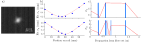
\includegraphics[width=\textwidth]{fig/lattice/dipole_profle_combo}
	\caption{a) Image taken from the InGaAs camera near the focus of a dipole beam.
	b) Beam waists along the rail as obtained from two-dimensional Gaussian fits to the images.
	c) Forward-propagation simulation of the beam waists which was designed to reshape the profiles.
	Cylindrical lenses only act on one of the axes, and are shown in a lighter blue.
	This iterative process produced the image on the left, with waist sizes 130$\mu$m and 124$\mu$m.}
	\label{fig:profiling}
	\end{figure}



	\begin{figure}
		\begin{minipage}{0.4\textwidth}
		\vspace{0cm}
		\caption{The $y$-axis dipole passes through a final focusing lens (lower middle) and is lifted by sturdy optics mounted to a heavy post.
	The upper mirror dials can be remotely controlled, using piezo-driven stepper motors, for precision alignment.
	The camera and refocusing optics for the absorption imaging system are just outside the left of the frame.}
		\label{fig:lifetime}
		\end{minipage}
		\hfill
		\begin{minipage}{0.6\textwidth}
		\vspace{0cm}
		\includegraphics[width=\textwidth]{fig/lattice/dipole_insertion_mirror} %20-11-17
		\end{minipage}
	\end{figure}



\subsubsection{Dipole trap}
\label{sec:dipole_trap}

	The dipole beams were first aligned to overlap with the magnetic trap with the use of resonant light piped through the dipole fibres.
	To do this, we redirected a few mW of light from the absorption imaging optics using a beamsplitter, passed it through an attenuator, and inserted it into the dipole optics via removable mirrors as illustrated in Fig.	\ref{fig:dipole_optics}.
	The endgame strategy was to achieve BEC by evaporative cooling in an optical dipole trap composed of two beams intersecting at right angles.
	This would require efficient transfer into the crossed dipole, which can be achieved by ensuring large mode overlaps between the initial and final traps \cite{MakingProbingUnderstanding}.	
	However, the spatial profile of the magnetic and dipole traps are very different, and so the principal means of achieving good transfer is to ensure the magnetic trap is very cold and tightly confined \todo{need to give numbers on this - what was your temperature in B trap, atom number, trap depth of ODT? etc}.
	Several iterations of magnetic field configurations and RF ramps were tried during the build.
	In the end, a key step forward was to install in-vacuum coils (at no small expense of effort) after I had left the lab.
	Details about the present trapping methods are presented in \cite{Abbas21}.
	This includes several re-assemblies of the optics and a change in the dipole trap configuration (namely switching to a second horizontal beam rather than a vertical beam as the upper flange of the Kimball chamber now hosts the coil feed-throughs including their cooling water).
	
	\todo{Short explanation of why the trap tightness matters.	What values did we ahve for the old coils?}
	However, the basic operation of the dipole is unchanged, including the alignment procedure we discovered, and so is documented here.
	As discussed above, the alignment procedure used resonant light, directed through the dipole fibre into the trap.
	Coarse alignment could be found by driving light near resonance through the dipole optics after loading a magnetic trap, and optimizing for the destruction of the cloud in response to the beam.
	Alignment could be finessed by reducing the intensity until the cloud recovers, then re-adjusting the beam to hit the centre of the trap and destroy it again.
	The cycle could be repeated until very low intensities were able to destroy the trap.
	Unfortunately we eventually found that there were multiple such optima.
	We determined that these were due to reflections of the beam from the inside of the chamber and scattering back across the trap.
	Afterwards, we acquired the image coincident with the resonant beam (rather than afterward) and found that when the beam intensity was reduced to a mere 4$\mu$W, the beam appeared to bore a hole through the cloud, as shown in Fig.	\ref{fig:dipole_align}.
	
	\begin{figure}
	\centering
	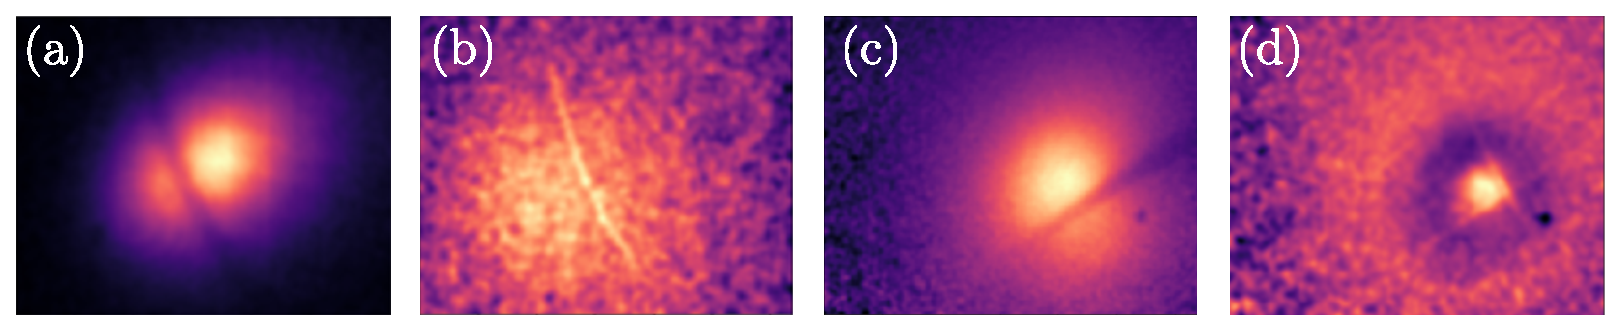
\includegraphics[width=\textwidth]{fig/lattice/dipole_alignment_stages}
		\caption{Stages of dipole beam alignment.
	The first alignment was achieved by passing resonant light through the cloud (a) and triggering the image acquisition (for 10 $\mu$s) at the same time as the resonant pulse.
	After switching to 1550nm light, the beam deflected slightly due to chromatic aberration in the optics (b) and could then be resolved in averages of 8-10 images. 
	The beam appears to bend in these images because the imaging beam was not aligned with the optical axis of the lenses, which was discovered and corrected using this technique.
	Some time later the vertical dipole was aligned using the same method (c) and so two dipoles could be loaded simultaneously. 
	Finally, an image of the combined magnetic and dipole traps could be taken ((d), average of 10 shots). To obtain this image, a Gaussian fit to the central cloud was subtracted from the image, with a residual halo and bright spot (c.f. the aforementioned issues with in-trap imaging).
	During my time in this lab, this was the best result we had for two dipoles.
	Absent more sensitive detection methods, it was not possible to determine when the dipoles had intersected and progress stalled here.}
	\label{fig:dipole_align}
	\end{figure}

	After this initial alignment several attempts were made to optimize the dipole loading by adjusting the final lens position, mirror orientation, and experimental control sequences.	
	Matters were made more difficult by several concurrent issues.
	For one, we were \emph{still} waiting for parts for the MCP-DLD detector mount, the ETP had since failed, and the CHT showed only modest changes in the ionization rate as a function of beam positioning.	
	This left absorption imaging as the sole means of ascertaining the loading efficiency.
	Unfortunately the signal-to-noise was poor and the dipole would only resolve after $\approx 8$ shots.
	At the time the experimental cycle was on the order of 15 seconds, and the long acquistion times were a major obstacle.
	It would eventually be found that the magnetic trap was simply not tight enough.
	The magnetic field gradient would later be improved by upgrade to in-vacuum coils during the tenure of the students who took up the mantle.
	

	% 	\com{Did we actually proceed in this manner? Why did we not build in the detector chamber right away? Or is the following more accurate: an issue that we were waiting on external contractors (right?) to produce some parts ({which?}) for the detector stack that would eventually be installed.
	% After initial delays in this delivery, we proceeded to install the detector chamber anyway to make continue development and testing?}
	% \rem{We were waiting on the MCP and wanted to test that we could achieve vacuum before installing them.
	%  Then since the absorption imaging worked, it was decided to proceed without the MCP DLD to test if the B trap, vacuum system etc worked.}
	% \begin{figure}
	% 	\centering
	% 	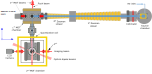
\includegraphics[width=\textwidth]{fig/lattice/abbas_schematic}
	% 	\caption{Schematic of the beamline, reproduced from \cite{Abbas21}.
	% The vacuum system was developed during the course of work described in this chapter, and has undergone several iterations since, including the addition of a coil (indicated) to maintain a magnetic quantization axis.
	% Not shown are many other developments including reconfigured optics, control system overhauls, rebakes, detector issues, building power failures, etc...}
	% % \end{figure}


	% % \begin{figure}
	% % 	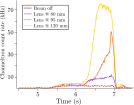
\includegraphics[width=0.5\textwidth]{fig/lattice/dipole_false_positive}
	% % 	\caption{A deceptive outcome.
	% \todo{Uncertain whether to include this.
	% It's sort of a fun cautionary tale, but discussing this red herring seems kind of unnecessary.
	% }}
	% % \end{figure}

	% %%%http://www.heliumbec.com/wiki/2017/08/16 MCS traces	evidence against dipole nature; various 'maxima', short steps led to large variation, diminishing peak shape over consecutive runs despite stable alignment and power etc - eventually found unexpectedly high N2 and CO2, perhaps some organic compound 'ablating' from the laser heat http://www.heliumbec.com/wiki/2017/10/20 and finally the 'idiot test' yes it still happened even with the He source off..
	
	% %%%We observe a weird problem that when the RF evaporator is set to the initial 500ms of 34MHz constant radiation, the frequency to the vertical dipole AOM shifts, causing the beam to move far enough that it no longer hits the fibre.	Further investigation show that this effect is present between 34-38MHz, but seems to disappear for 33MHz and below as well as 40MHz.	Oddly though, for the higher initial frequencies hen the ramp is swept through the trouble region we see no deviation (although it might be too quick to observe).	Anyway, for now we just set the initial frequency at 33MHz and move on, and will investigate further some other day.	http://www.heliumbec.com/wiki/2017/07/03 first crack sighting	Noting when effect no longer visible gives size estimate of the cloud can be used to cross-check with the absorption imaging.
	% Dipole doesn't show up in same place as the refractive indices are different.


	%%%http://www.heliumbec.com/wiki/2017/10/26 first sighting of dipole - abandoned idea of optimizing on ion signal and just took a ton of images while stepping through focus lens posn

	%Waists are 73 and 55 micron respectively, crossing the centre of the biased trap, 6mm above the centre of the horz coils
	% Trap freqs 1.1,1.2,1.7 kHz and 150muK deep

\section{Progress and outlook}
	
	After my departure, the lab sat motionless for some months as I had been the sole graduate student on the project.
	Later, the \mhe lattice team was renewed by two PhD students (A. H.	Abbas and X. Meng) and a Masters student (R. S. Patil).
	The team has since achieved a BEC production time of as low as 3.3 seconds, nearly a factor of 2 faster than the prior art \cite{Bouton15} and a factor of 8 faster than the BiQUIC machine.
	The subsequent publication \cite{Abbas21} contains details about the new coils, additional infrastructure and cooling techniques, and characterization techniques.
	The large condensates, containing something on the order of a million atoms, are also competitive with the state-of-the art.
	I take my hat off to the students who picked up the trail where I had left off, and accomplished a goal I'd struggled towards for two years.
	

	% \begin{figure}
	% 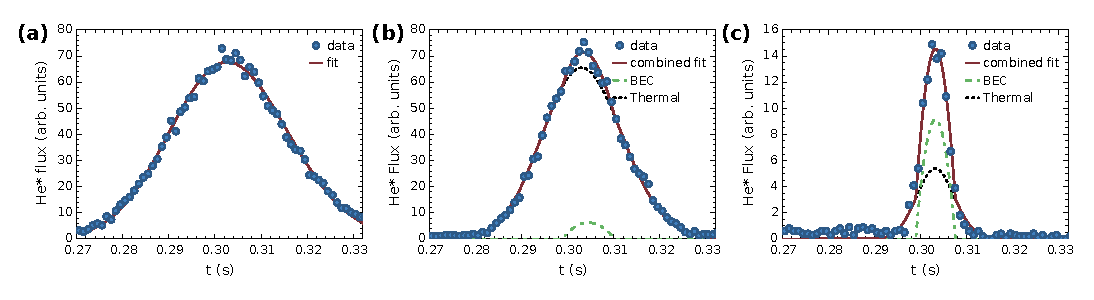
\includegraphics[width=\textwidth]{fig/lattice/abbas_tof}
	% \begin{minipage}{0.45\textwidth}
	% \vspace{0pt}
	% 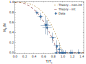
\includegraphics[width=\textwidth]{fig/lattice/abbas_Tc}
	% \end{minipage}
	% \hfill
	% \begin{minipage}{0.55\textwidth}
	% 	\vspace{0pt}
	% 	\caption{Top: Onset of condensation in the time-of-flight profile recorded on the MCP-DLD detector stack, reproduced from \cite{Abbas21}.
	% In the case of colder clouds, the thermal fraction can get so small and cold that it is not visible under the thomas-fermi profile.
	% Left: The condensed fraction versus the temperature obtained by fitting the thermal part.
	% The data agree very well with the predictions including the effect of inter-atomc interactions, which shifts the critical temperature down by about 10\% in this configuration.}
	% % \end{minipage}
	% % \end{figure}


	% % \begin{figure}
	% % 	\includegraphics[width=\textwidth]{fig/lattice/new_coils.png}
	% % 	\caption{New installations since my time in the lab.
	% Top: The new in-vacuum coils (illumated by flashlight, lower right) and MCP-DLD detector stack mounted in vacuum at the pico-torr level (bottom).}
	% % 	\includegraphics[width=\textwidth]{fig/lattice/DLD_in_vacuum}
	% % \end{figure}


	% Ahead, the team is faced with the challenge of aligning and optimizing three pairs of lattice beams.
	% \todo{Talk about some of the Bose-Hubbard physics before the additional upgrades}.
	% Beyond that, there lies a fork in the road.
	% One path leads to the Fermi-Hubbard model by way of further infrastructure upgrades to achieve degenerate $^3$\mhe in the same machine.
	% The expertise gained through the ongoing upgrade of the BiQUIC machine would be instrumental in this mission.
	% The other path is towards the study of the disordered Bose-Hubbard model (also known as the Aubry-Andr\'{e} model), which has been studied in quantum gas microscopes \cite{Rispoli} but not, so far, with measurements of single-particle momentum.
	% Theoretical studies that momentum-space localization occures in incommensurate lattices (which approximate a random lattice by superposing two lattices whose wavelengths are not related by a low-order rational number) \cite{Larcher11}.
	% The momentum-space aspects of many-body localization and thermalization have been less well explored in optical lattices.




% Well, dipole, maybe better automation, certainly better envt controls...
% New coils, solder catastrophe, new plates \#\# Issues/What next
% Stability: Vibration, temp, vacuum Optics: Power, profile Automatic
% optimization Broad goals Fermions Quasirandom lattices Are these
% actually resources or what? Next generation laser tech?


	% 1e6 atoms in BEC!
		% Small coils, fast switching times
		% 5 turn Anti helmholtz coils, 40mm diameter centred on Y
		% 8 turn bias coil in Z
		% Internally cooled coils, 2/0.4mm diameter
		% 120A through quad AH and 62A through bias, switched by fatass mosfet?
		% 89x89x57 Hz
		% Cracked CHT?
		% The soldering incident


	% % 5W fibre amp for cooling beam


% Due to aforementioned universality properties, can abstract away a wide class of materials perhaps even including properties that don't exist naturally or have yet to be engineered.
% 	Can then iterate towards optimal function in this simulacrum and then (with just as much work) translate back to materials....
% 	insertion of 'agents' directly into a synthetic physical envt
% 	Any examples of this happening yet?

	
	% % 1D Doppler cooling [tychkov paper 25], with .01Isat and sigma+ polz directed vertically down along the bias direction.
		% Detuned -Gamma/2.
		%  After 500mss have 4.9e7 atoms at 83\mu K.
	
	
	% % QUIC trap linearly relazed to an unbiased trap with 1.1G/cm gradient and then switched off with a FET.
	% Additional square coil is switched on to create a uniform 1.6G field pointing in z direction.
	% Turned on before the QUIC rampdown starts.
	% Eventually found that the earth's field was sufficient to maintain the quantiation axis and suppress Penning ionization, so is switched off after 700ms in ODT.
	% Measure 5e6 atoms at 13.5muK, 0.5 PSD
	% % Trap depth reduced by exponential rampdown of power over 1 sec.



	% % Second MOT gradient 4.4G/cm (in weak or strong axes?)
	% % 451mm fall to detector
	% % 	DLD not operational yet so measure the current pulses on the plates frmo the charge depletion when atoms impact the plates.
	% Fast amplifier and a discriminator then recorded using a digital counter to extract 1D tof distribution.
	% Compressed MOT sequence
		% % MOT compression - ramps to 1.42G/cm in 10ms while linearly ramping lasers to -0.4Gamma and decreasing intensity by a hundredfold, then switching off and the +1s remain trapped
		% % Then compress the mag trap to 16.6G/cm in 100\mu s, and ramp the bias up in 100ms to provide a 10G bias in the QUIC trap.
		% Has radial 89Hz and 57Hz z freqs.
		% Have 5.3e7 atoms at 0.44mK.
			% Measured using absorption imaging along the x axis using an InGaAs CCd.
			% Flipper mirrors allow operation on the MOT axis but mean imaging not available during MOT.

